%%%%%%%%%%%%%%%%%%%%%%%%%%%%%%%%%%%%%%%%%
% Tufte-Style Book (Minimal Template)
% LaTeX Template
% Version 1.0 (5/1/13)
%
% This template has been downloaded from:
% http://www.LaTeXTemplates.com
%
% License:
% CC BY-NC-SA 3.0 (http://creativecommons.org/licenses/by-nc-sa/3.0/)
%
% IMPORTANT NOTE:
% In addition to running BibTeX to compile the reference list from the .bib
% file, you will need to run MakeIndex to compile the index at the end of the
% document.
%
%%%%%%%%%%%%%%%%%%%%%%%%%%%%%%%%%%%%%%%%%

%----------------------------------------------------------------------------------------
%	PACKAGES AND OTHER DOCUMENT CONFIGURATIONS
%----------------------------------------------------------------------------------------

\documentclass[justified, openany, notoc]{tufte-book} % Use the tufte-book class which in turn uses the tufte-common class

\hypersetup{colorlinks} % Comment this line if you don't wish to have colored links

\usepackage{microtype} % Improves character and word spacing
\usepackage{amsmath}
\usepackage{bm}
\usepackage{empheq}
\usepackage{lipsum} % Inserts dummy text
\usepackage[scientific-notation=true]{siunitx}
\usepackage{booktabs} % Better horizontal rules in tables
\usepackage{caption}
\usepackage{subcaption}
\usepackage{graphicx} % Needed to insert images into the document
\graphicspath{{graphics/}} % Sets the default location of pictures
\setkeys{Gin}{width=\linewidth,totalheight=\textheight,keepaspectratio} % Improves figure scaling

\usepackage{fancyvrb} % Allows customization of verbatim environments
\fvset{fontsize=\normalsize} % The font size of all verbatim text can be changed here

\newcommand{\hangp}[1]{\makebox[0pt][r]{(}#1\makebox[0pt][l]{)}} % New command to create parentheses around text in tables which take up no horizontal space - this improves column spacing
\newcommand{\hangstar}{\makebox[0pt][l]{*}} % New command to create asterisks in tables which take up no horizontal space - this improves column spacing
\newcommand{\paren}[1]{\left( #1 \right)}
\newcommand{\bracket}[1]{\left[ #1 \right]}
\usepackage{xspace} % Used for printing a trailing space better than using a tilde (~) using the \xspace command
\usepackage{float}
\newcommand{\monthyear}{\ifcase\month\or January\or February\or March\or April\or May\or June\or July\or August\or September\or October\or November\or December\fi,\space\number\year} % A command to print the current month and year
\newcommand{\openepigraph}[2]{ % This block sets up a command for printing an epigraph with 2 arguments - the quote and the author
\begin{fullwidth}
\sffamily\large
\begin{doublespace}
\noindent\allcaps{#1}\\ % The quote
\noindent\allcaps{#2} % The author
\end{doublespace}
\end{fullwidth}
}

\newcommand{\blankpage}{\newpage\hbox{}\thispagestyle{empty}\newpage} % Command to insert a blank page

\usepackage{makeidx} % Used to generate the index
\makeindex % Generate the index which is printed at the end of the document

%----------------------------------------------------------------------------------------

\renewcommand{\maketitlepage}{%
\thispagestyle{empty}
\begin{fullwidth}
\begin{center}
  \vspace*{1cm}

  \textbf{\Huge Implementation of the AK-MCS algorithm for structural reliability}
       
  \vspace{1cm}

  \textbf{by} \\

  \textbf{\large Juan Camilo Lugo Rojas}

  \vspace{2cm}
  \textbf{Advisor} \\
  \textbf{\large Dr. techn. Diego Andrés Alvarez Marín}

  \vspace{1.5cm}

  
  
\includegraphics[width=0.4\textwidth]{graphics/escudo}
  
  \vfill
  \textit{Submitted in partial fulfillment of the requirements\\
  for the degree of}

  \vspace{0.2cm}

  \large Civil Engineer

  \vspace{0.8cm}

  Department of Civil Engineering\\
  Faculty of Engineering and Architecture\\
  National University of Colombia at Manizales\\
  \vspace{0.5cm}

  \monthyear
       
\end{center}
\end{fullwidth}
}

% chapter title style
\definecolor{chapcolor}{rgb}{0.447, 0.035, 0.337}
\def\Vhrulefill{\leavevmode\leaders\hrule height 0.8ex depth \dimexpr0.4pt-0.7ex\hfill\kern0pt}

\setcounter{secnumdepth}{2}

\titleformat{\chapter}[display]%
  {\Huge\rmfamily\itshape\bfseries}
  {{\colorbox{chapcolor}{\parbox{2cm}{\centering\itshape\Large\color{white}Chapter \thechapter}}}\Vhrulefill}{0pt}
  {}

% toc

\setcounter{tocdepth}{2}
\addtocontents{toc}{\itshape}

\begin{document}

\frontmatter

%----------------------------------------------------------------------------------------

\maketitle % Print the title page

%----------------------------------------------------------------------------------------
%	DEDICATION PAGE
%----------------------------------------------------------------------------------------

% \cleardoublepage
% \thispagestyle{empty}
% ~\vfill
% \begin{doublespace}
% \noindent\fontsize{18}{22}\selectfont\itshape
% \nohyphenation

% \end{doublespace}
% \vfill
% \vfill

%----------------------------------------------------------------------------------------
%	Abstract
%----------------------------------------------------------------------------------------
%\cleardoublepage
\chapter*{Abstract} % The asterisk leaves out this chapter from the table of contents
A study of the AK-MCS method is presented, which seeks to optimize the determination of failure probabilities by means of Monte Carlo Simulations. A review of key concepts of structural reliability is made, in order to contextualize the field of application of the studied algorithm. A theoretical review of the Gaussian Process Regression is made to be able to understand the AK-MCS algorithm. Finally, several models are implemented, comparing the performance of AK-MCS with that of classical Monte Carlo Simulations. \\

\textbf{Keywords:} Monte Carlo Simulation, Structural Reliability Analysis, Krigin Regression, Active learning methods.

\cleardoublepage
\chapter*{Resumen} % The asterisk leaves out this chapter from the table of contents
Se presenta un estudio del método AK-MCS, el cual busca optimizar la determinación de probabilidades de falla mediante las Simulaciones de Monte Carlo. Se hace una revisión de conceptos clave de confiabilidad estructural, con el fin de contextualizar el campo de aplicación del algoritmo estudiado. Para poder entender AK-MCS, se hace una revisión teórica de las regresiones mediante procesos gaussianos. Finalmente, se implementan varios modelos, comparando el desempeño del algoritmo estudiado, con el de las simulaciones de Monte Carlo clásicas. \\

 \textbf{Palabras clave:} Simulación de Monte Carlo, Análisis de confiabilidad estructural, Regresión Kriging, Métodos de aprendizaje activo.
%----------------------------------------------------------------------------------------
\pagenumbering{roman}
\tableofcontents % Print the table of contents

%----------------------------------------------------------------------------------------

\listoffigures % Print a list of figures
\addcontentsline{toc}{chapter}{List of Figures}
%----------------------------------------------------------------------------------------
\addtocontents{}{}
\listoftables % Print a list of tables
\addcontentsline{toc}{chapter}{List of Tables}
%------------------------------------------------


%----------------------------------------------------------------------------------------

\mainmatter
\pagenumbering{arabic}

%----------------------------------------------------------------------------------------
%	CHAPTER 1
%----------------------------------------------------------------------------------------

\chapter{Introduction}
\label{ch:1}

The study of the behavior of a structure given the properties of its materials, its geometric configuration, and the loads to which it is subjected is known as structural analysis. Within this field, it is of particular interest to determine when a structure exceeds certain levels of distress that can lead to collapse, considerably affect its performance, or affect its serviceability, among other criteria. These are known as limit states \citep{Melchers2018}. \\

The determination of whether these limits have been exceeded has been addressed from different perspectives throughout history. When the variables involved are considered to take unique values, we have what is known as the deterministic approach. There is a natural extension of the latter, which consists of considering that the values of these variables present variations derived from their intrinsic uncertainty, this being known as the probabilistic approach \citep{Ditlevsen1996}. \\

The term reliability is commonly defined as the complement of the probability of failure (failure being understood as the exceeding of a predefined limit state). In other words, reliability corresponds to the probability that the structure will function properly during a period of time \citep{Melchers2018}. \\

Several methods have been derived from MCS, trying to overcome the problem of
its computational cost, while preserving its strengths. In this document we study
one of those methods, known as AK-MCS for Active learning reliability method combining
Kriging and MCS, which attempts to obtain results equivalent to those given by MCS in a 
more efficient manner \citep{Echard2011}.

\section{Motivation}
The fundamental reason for doing this project is the desire to be initiated in academic
research, which contributes to the generation of knowledge and the development of 
science and the self.\\

Additionally, the structural reliability assesment is a very fascinating field which 
is constantly developing and can have a great impact. I can visualize myself working on these 
topics in the future.
\section{Objective}
The main objective of this final project is to implement the algorithm described in 
an article\cite{Echard2011} that proposes a new approach based on MCS and Kriging
metamodel to asses structural reliability. In order to satisfactorily do this, many
specific objectives have to be achieved, which include:
\begin{itemize}
    \item Learning the Monte Carlo Simulation method.
    \item Learning the Kriging regression algorithm.
    \item Reading and completely understand the article.
    \item Implementing the previously mentioned methods in Python.
    \item Reviewing articles that aim to improve the performance of the AK-MCS algorithm.
    \item Evaluating the performance of the algorithm, comparing it with the basic MCS.
\end{itemize}


%----------------------------------------------------------------------------------------
%	CHAPTER 2
%----------------------------------------------------------------------------------------
\chapter{Some concepts of Structural Reliability}
\label{ch:2}
\section{Reliability problem formulation}
The reliability problem is based on the performance function $G(\bm{x})$ defined as:
\begin{equation} \label{eq:1}
    G(\bm{x})=R(\bm{x}) - S(\bm{x})
\end{equation}

where $\bm{x}$ is the vector of input variables, in which are included the geometric and material properties, as well as the acting loads, and in general all the variables taken into consideration that affect the behavior of the structure; $S(\bm{x})$ is a load effect acting on the structure, and $R(\bm{x})$ is its capacity to withstand it. The limit state equation corresponds to $G(\bm{x})=0$, i.e. when the acting and resisting forces are equal. A violation of the limite state occurs when $G(\bm{x}) \leq 0$, otherwise (when $G(\bm{x}) > 0$), we say that the structure is safe. \\

For complex problems, the performance function usually cannot be expressed as in \ref{eq:1}, but in the form:

\begin{equation}
    G(\bm{x}) = r(\bm{x}) - \hat{r}
\end{equation}
where $r(\bm{x})$ is an implicit function and $\hat{r}$ is a critical threshold. $r(\bm{x})$ can be, for instance, the result obtained from a finite element analysis. \\

The objective is to determine the probability of failure $p_f$ of the structure:
\begin{equation} \label{eq:pf}
p_f = P[G(\bm{x}) \leq 0]    
\end{equation}

\begin{testexample}[Cantilever beam]
Consider the beam shown in figure \ref{fig:beam}, with rectangular cross section of base $b$ and height $h$. A performance function can be defined as follows:
\begin{equation} \label{eq:example}
    G(\bm{x})=R - \underbrace{\frac{6PL}{bh^2}}_{\sigma_b}
\end{equation}


where $\sigma_b$ is the maximum bending stress to which the beam is subjected and $R$ is the beam resistance. Then we have that if $G(x) \leq 0$, i.e. if $R \leq \sigma_b$, the beam will fail according to this criterion.
\end{testexample}

\begin{marginfigure}[-12\baselineskip]
    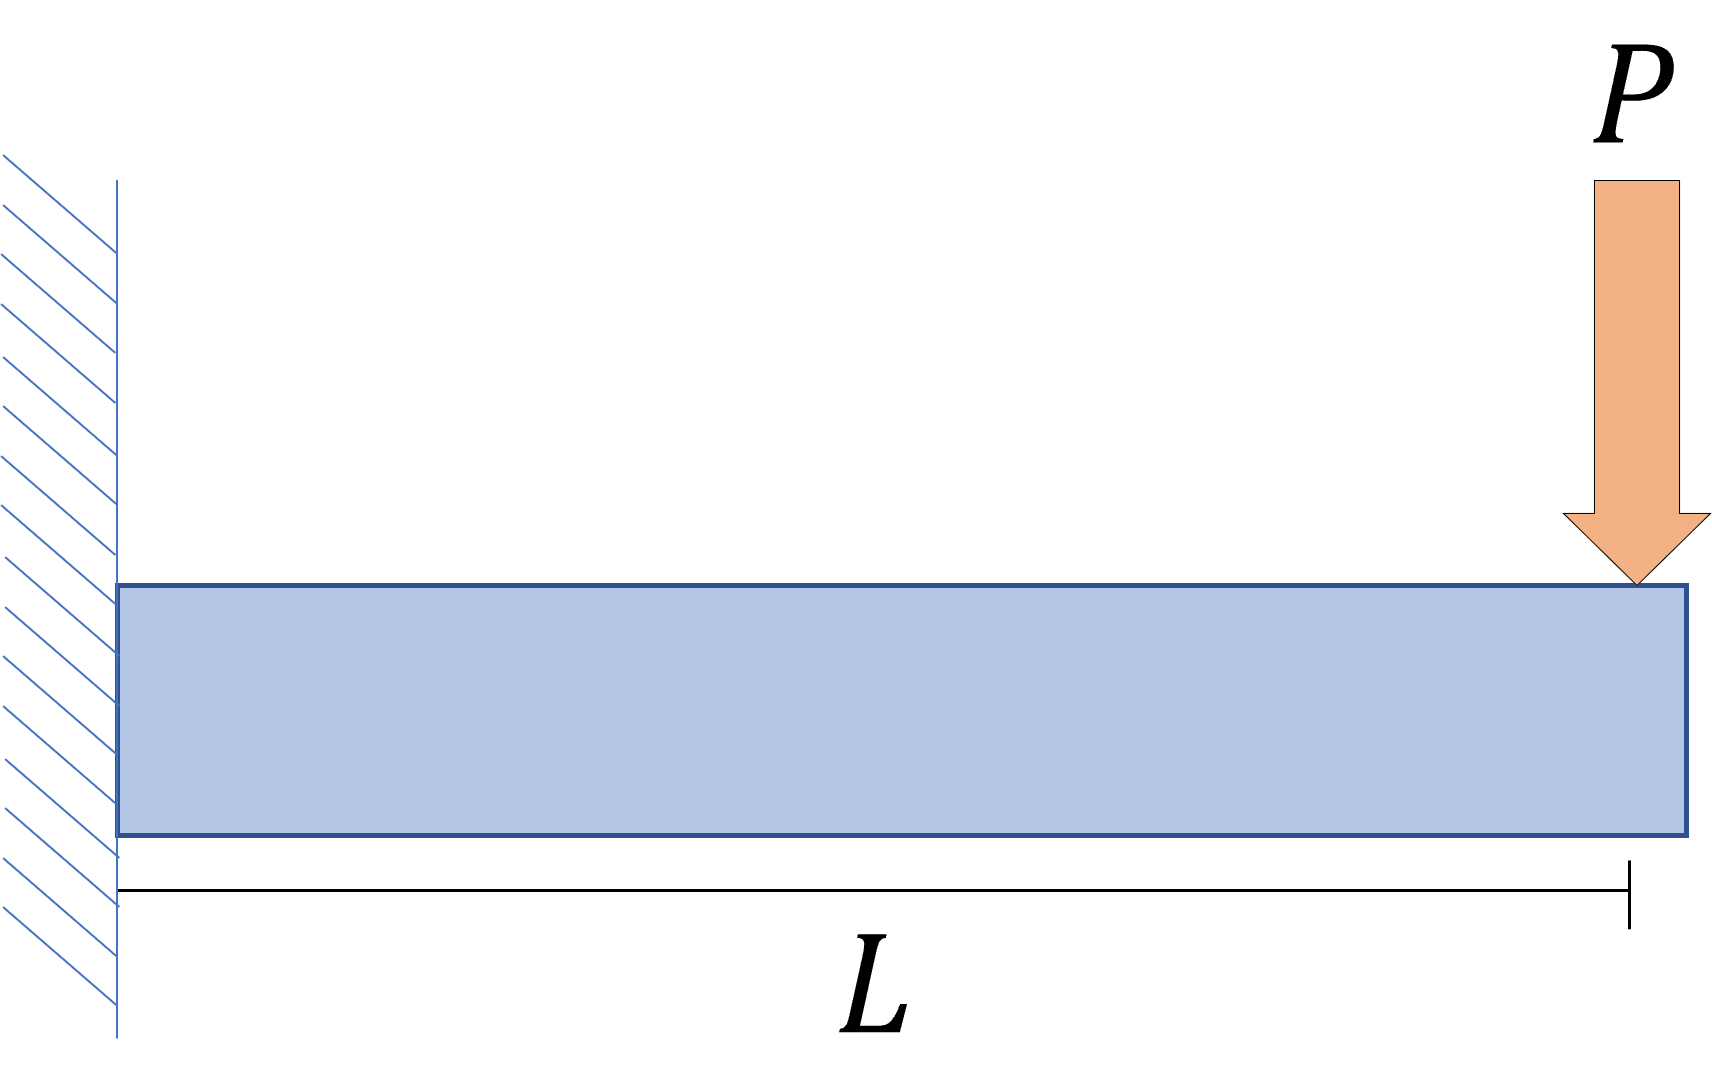
\includegraphics[width=\linewidth]{beam.png}
    \caption{Cantilever beam.}
    \label{fig:beam}
\end{marginfigure}


\section{Realiability assessment approaches}

\subsection{Deterministic approach}
The deterministic approach is the traditional one. In this approach, the uncertainties
in the forces and resistances are covered by assuming that the variation of these
forces and resistances have limits that are not exceeded. Given this simplicity,
it is usually necessary to overestimate the magnitudes in order to provide greater
safety. This is usual in design codes when considering safety factors in the limit
state equations. It is widely used, especially in simple and common problems.
However, this required safety margin implies the need to assume higher costs. \\

In this case, the result of the formula \ref{eq:pf} is either $1$ or $0$, since the values of the variables are considered fixed, thus the inequality is either fulfilled or not.
\begin{testexample}[Cantilever beam (cont.)]
In order to design the beam in such a way that it does not violate the limit state equation considering this approach, design parameters are selected such that $G(\bm{x}) > 0$. For safety reasons, in the equation \ref{eq:example}, $\sigma_b$ is replaced by $\hat{\sigma}_b = \lambda \sigma_b$, being $\lambda \geq 1$ the safety factor, which is determined empirically based on previous experience with similar problems. \\

Although the limit state is not violated, failure may still occur, due to the uncertainty that is ignored.
\end{testexample}
\subsection{Partial probabilistic approach}
The historical record of events that expose structures to large loads, such as
earthquakes, floods, tornadoes, etc., shows that they have a certain frequency
according to their magnitude. For instance, during one day there may be multiple
low-scale earthquakes, but every few years there is one of considerable destructive
power. \\

The partially probabilistic approach handles these return periods when considering
the maximum loads to which a structure will be subjected during certain period of time. This allows the selection of design parameters in accordance with the expected service life of the structure, seeking a balance between the probability of failure and the costs that may be incurred. \\

It can be seen that some randomness is considered when accounting for the variability over time of the loads; however, this approeach does not acknowledge that even at a given instant there is uncertainty.

\begin{testexample}[Cantilever beam (cont.)]
    In this case, to estimate $\hat{\sigma}_b$, the historical records of the values taken by the applied load $P$ are considered to study the frequency of events in which it takes very high values. Then a value of $P$ is selected, attempting to maintain a good balance between the costs and the risk of failure. \\
    
    There is a return period associated with the magnitude of $P$ chosen, which accounts for the probability that the structure will fail during a certain period of time.
\end{testexample}

\subsection{Probabilistic approach}
The variables involved in the performance function can be considered random. For this purpose, through statistical data and experience, the distribution that each of them follows is determined. \\

Let consider the case when $G(\bm{x})$ can be expressed as in \ref{eq:1}. It is possible to obtain probability density functions $f_R(x)$ and $f_S(x)$ that describe $R$ and $S$ respectively. Since the limit state is violated when $G(\bm{x}) \leq 0$, the probability of failure can be roughly represented by the overlap of $f_R(\bm{x})$ and $f_S(x)$ as shown in figure \ref{fig:frfs}. \\

\begin{marginfigure}[-12\baselineskip]
    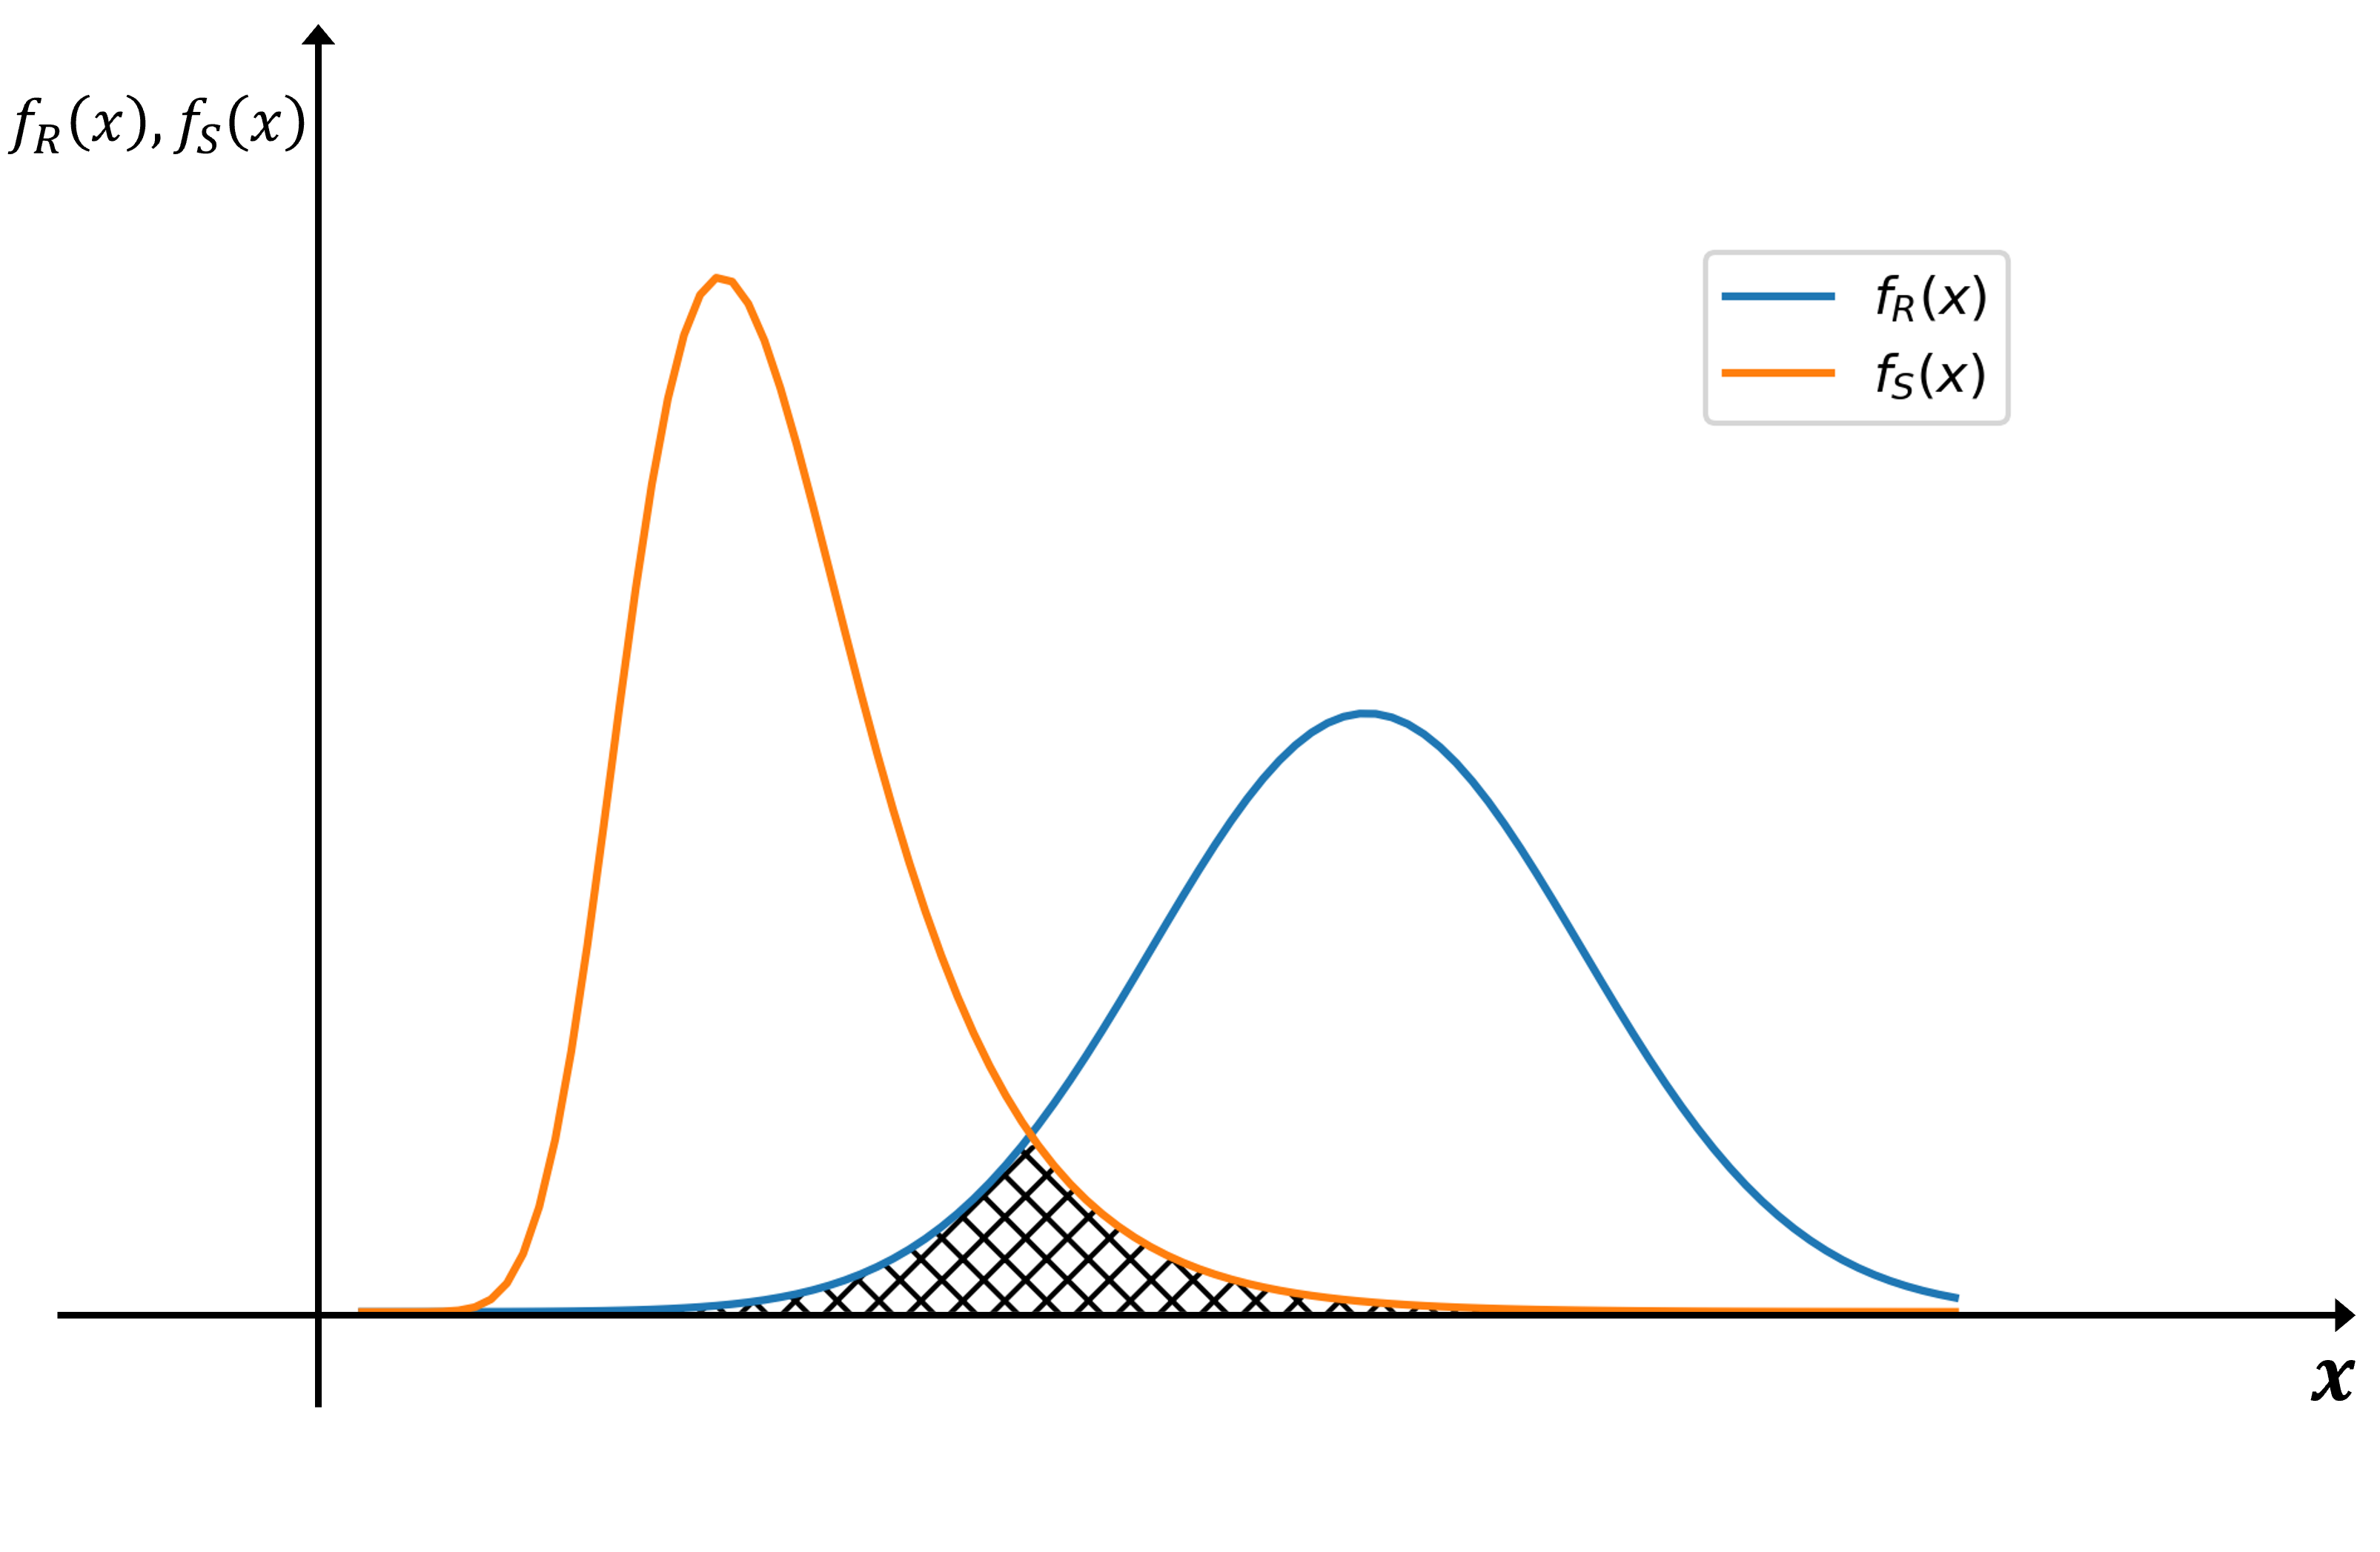
\includegraphics[width=\linewidth]{frfs.png}
    \caption{Representation of $p_f = P\bracket{R(\bm{x}) \leq S(\bm{x})}$}
    \label{fig:frfs}
\end{marginfigure}

When $f_R(x)$ and $f_S(x)$ are independent, the probability of failure can be expressed as:

\begin{equation}
    p_f = \int_{-\infty}^{\infty} F_R(x)f_S(x)\mathrm{d}x
\end{equation}

which is known as a convolution integral, where $F_R(x)$ is the probability that $R \leq x$, so by considering its product with $f_S(x)$ over all possible values of $x$, $p_f$ is obtained. \\

In the general case, the probability of failure is given by:

\begin{equation} \label{eq:pfint}
    p_f = \underset{G(\bm{x})\leq 0}{\int \cdots \int}f_{\bm{x}}(\bm{x})\mathrm{d}\bm{x}
\end{equation}

where $f_{\bm{x}}(\bm{x})$ is the joint probability density function of the considered variables $\bm{x}$. The solution of \ref{eq:pfint} can be tricky. For this purpose, several methods have been developed, some of which will be reviewed in the following section.

\section{Reliabiliy assessment methods}

The analysis methods used to estimate \ref{eq:pfint} can be divided into two main categories: analytic and synthetic. The former are based on the Taylor series expansion of the limit state function, while the latter require the generation of random samples of the variables associated with the model. In this section we will review some generalities of these two categories, their applicability and limitations, with a particular focus on the latter, to which the method reviewed in this document corresponds.

\subsection{Analytic methods (FORM and SORM)}
The \textit{First} and \textit{Second Order Reliability Methods} require the transformation of the vector $\bm{x}$, defined by their joint density function $f_{\bm{x}}$, into a set of normally distributed independent variables $\bm{u}$. The Taylor series expansion of $G(\bm{u})$ is considered, of first order when using FORM, and of second order in the case of SORM. Iteratively, it is obtained the denominated design point $\bm{u^*}$ by minimizing its distance from the origin such that $G(\bm{u*})=0$. By considering the Taylor series expansion at the design point, a hyperplane is obtained, such that it divides the design space (the possible values taken by the input variables) into the failure and the safe domain. \\

As these methods require the calculation of the gradient of the performance function, in addition to the Hessian matrix in the case of SORM, the practicality of their application depends heavily on the form of the performance matrix, greatly increasing the complexity of the calculations when the dimensionality of the problem increases. \\

\subsection{Synthetic methods (Monte Carlo Simulation)}
Reliability analysis using MCS consists of generating samples in the design space that are used to evaluate the structural model and thus numerically estimate the probability of failure. \\


To generate the sample, random numbers are first generated. Several algorithms have been developed for this purpose, seeking to generate samples uniformly distributed between 0 and 1. Nowadays, the most widely used algorithm is the Mersenne Twister (see \citep{MT}). Starting from the uniformly distributed numbers, the sample is generated following the given distributions. The most general technique for this is the inverse transform method. For some particular distributions there are more efficient methods, for example, for a normal distribution the Box and Muller algorithm (see \citep{BM}) can be used. \\

The equation \ref{eq:pfint} can be written as: 

\begin{equation} \label{eq:pfmc}
    p_f = \int \cdots \int I\bracket{G(\bm{x}) \leq 0}f_{\bm{x}}(\bm{x})\mathrm{d}\bm{x}
\end{equation}

where $I\bracket{G(\bm{x}) \leq 0}$ is an \textit{indicator function} defined as:
\begin{equation}
I\bracket{G(\bm{x}) \leq 0} = 
\begin{cases}
1, \quad \text{if } G(\bm{x}) \leq 0 \\ 
0, \quad \text{if } G(\bm{x}) > 0
\end{cases}
\end{equation}

But equation \ref{eq:pfmc} corresponds to the expected value of $I\bracket{G(\bm{x}) \leq 0}$, so considering a generated sample of $n_{MC}$ elements, being $\bm{\hat{x}}_j$ an element of the sample, it follows that the probability of failure can be approximated as:

\begin{equation}
    p_f \approx \frac{1}{n_{MC}} \sum_{j = 1}^{n_{MC}} I\bracket{G(\bm{\hat{x}_j}) \leq 0}
\end{equation}

This estimated value of $p_f$, since it depends on a random sample, can vary considerably. A measure of such variation is the coefficient of variation, which is defined as:

\begin{equation}
    \text{C.O.V}_{p_f} = \sqrt{\frac{1-p_f}{p_f \; n_{MC}}}
\end{equation}

Note that the C.O.V is smaller when the $p_f$ is larger, as the relative variation it can have is smaller; and it can also be reduced by using a larger number of samples. \\

Among the main advantages of MCS is that it makes no assumptions about the limit state function, so it is not necessary to perform any kind of transformation to the design space. In addition, it does not present as many drawbacks as other methods when dealing with high dimensionality problems. However, its main drawback is its computational cost. When having very complex limit state functions, it is necessary to evaluate it too many times to obtain an accurate enough result. Variations of the method are continuously being developed to deal with this problem.The AK-MCS algorithm, which is explained in the next chapter, is one of these variations.

%----------------------------------------------------------------------------------------
% \chapter{Reliability Assesment}
\label{ch:3}
\chapter{The AK-MCS algorithm}
\label{ch:5}
Crude Monte Carlo Simluations are easy to implement and robust in dealing with 
reliability problems. However, they require the evaluation of the expensive performance
function a considerable amount of times. AK-MCS\sidenote{stands for Active learning method combining Kriging and
Monte Carlo Simulation and is described in
\citep{Echard2011}}, that  and must be seen as a modification of the traditional MCS,
aims to overcome this downside making use Gaussian Processes
Regressions and a learning function to optimize the number of calls of the performance function
on a Monte Carlo simulation.
\section{Preliminaries}
\subsection{Gaussian Identity of conditional distributions}
The joint probability density of the multivariate Gaussian distribution is given by:
\begin{equation}
  p(\bm{x}|\bm{m},\bm{\Sigma}) = (2\pi)^{D/2}|\bm{\Sigma}|^{-1/2}\exp{\left(-\frac{1}{2}(\bm{x}-\bm{m})^{T}\bm{\Sigma}^{-1}(\bm{x}-\bm{m})\right)}
\end{equation}
where $\bm{x}$ is a vector of length $D$, $\bm{m}$ is the mean vector, and $\bm{\Sigma}$ is the covariance matrix, which is symmetric and positive definite. To say that $\bm{x}$ follows a Gaussian distribution with mean  $\bm{m}$ and covariance $\bm{\Sigma}$ we write $\bm{x} \sim \mathcal{N}(\bm{m}, \bm{\Sigma})$. \\

Let $\bm{x}$ and $\bm{y}$ be jointly Gaussian random vectors
\begin{equation}
  \begin{bmatrix}
    \bm{x} \\ \bm{y}
  \end{bmatrix}
  \sim \mathcal{N}\left(
    \begin{bmatrix}
    \bm{\mu_x} \\ \bm{\mu_y}
    \end{bmatrix} , \begin{bmatrix}
      \bm{A} & \bm{C} \\ \bm{C}^T & \bm{B}
    \end{bmatrix} \right)
\end{equation}

then the conditional distribution of $\bm{x}$ given $\bm{y}$ is:
\begin{equation}
  \bm{x}|\bm{y} \sim \mathcal{N}\left(\bm{\mu_x} + \bm{C} \bm{B}^{-1}(\bm{y}-\bm{\mu_y}), \; \bm{A} - \bm{C}\bm{B}^{-1}\bm{C}^T \right)
\end{equation}
The proof of this fact can be detailed in \citep{Bishop}, section 3.1.

\subsection{Gaussian Processes}
A Gaussian process, is a collection of random variables, any finite number of which have a joint Gaussian distribution. It is completely specified by its mean function and covariance function.

\begin{equation}
  f(\bm{x}) \sim \mathcal{GP}(m(\bm{x}), k(\bm{x}, \bm{x'}))
\end{equation}

\begin{equation}
  \begin{bmatrix}
    \bm{y} \\ \bm{\mathrm{f}}_*
  \end{bmatrix}
  \sim \mathcal{N}\left(
  \bm{0}, \begin{bmatrix}
      \bm{K}+\sigma_n^2 \bm{I} & \bm{K}_* \\ \bm{K}_*^T & \bm{K}
    \end{bmatrix} \right)
\end{equation}
\section{Step-by-step of the method}
\begin{enumerate}
    \item \textbf{Generation of a Monte Carlo population in the design space.}
    According to the involved random variables, this population named $S$ of $n_{MC}$ points 
    is generated.
    \item \textbf{Definition of the initial design of experiments (DoE).} The initial
    DoE consists of a random selection of $N_1$ points of $S$. It is preferred to be
    small, adding at each iteration only the point that improves the metamodel
    the most. We will be using a dozen points as suggested in \citep{Echard2011}.
    \item \textbf{Computation of the Kriging model.} The Kriging regressor is trained
    with the performance function $G$ evaluated on the initial DoE. A model with an
    squared-exponential kernel is used.
    \item \textbf{Prediction by Kriging and estimation of the probability of failure.}
    Predictions of the performance function over the Monte Carlo population, $\widehat{G}(x_i)$
    for $i = 1, ..., n_{MC}$ are made with the previously trained Kriging model. 
    Then, the estimated probability of failure $\widehat{p_f}$ is obtained by calculating the ratio
    of the points $x_i \in S$ such that $\widehat{G}(x_i) \leq 0$, i.e.:
    \begin{equation}
        \widehat{p_f} = \frac{n_{\widehat{G}(x_i) \leq 0}}{n_{MC}}
    \end{equation}
    \item \textbf{Identification of the best next point in $S$ to be evaluated on the
    performance function.} At this stage, the learning function is computed for each
    point of $S$ to determine the next point that should be added to the DoE to
    improve the most the metamodel.
    \item \textbf{Evaluation of the stopping condition.} The stopping condition
    associated to the learning function is evaluated for the point selected in the
    previous stage. If the criterion is met, we skip to Stage 8. Otherwise, we
    continue with Stage 7.
    \item \textbf{Update of the design of experiments.}
    The point identified at stage 5 is added to the current DoE, such that $N_{i+1} = N_i + 1$.
    Then, the method goes back to Stage 3.
    \item \textbf{Computation of the coefficient of variation of the probability of
    failure} If the stopping condition is satisfied, the metamodel is said to be
    accurate enough on the sign of the performance function on $S$. Subsequently,
    it is checked if $S$ is large enough to obtain a low coefficient of variation
    on the estimation of $p_f$. If the coefficient of variation is lesser than
    $5\%$, AK-MCS stops and the last estimation of the probability of failure is
    considered as the result. In other case, it continue to Stage 9.
    \item \textbf{Update of the population.} $S$ is increased with other $n_{MC}$ points from the
    design space generated in the same way that in Stage 1, and proceed back to stage 3.
\end{enumerate} 

\section{Learning Functions}
The learning functions are used to decide the next point of the population to be
included in the DoE. In order to do that, they give a score to each $x_i$ of $S$
according to the value $\widehat{G}(x_i)$ and by its variance $\sigma^2_{\widehat{G}}(x_i)$
given by the Kriging regressor. Every learning function comes along with a learning criterion
and with a stopping condition on the obtained scores.

\subsection{Expected feasibility function (EFF)}
It is defined as
\begin{align}
    EFF(x)= \paren{\widehat{G}(x) - a}& \paren{2 \Phi (C) - \Phi (C^+) - \Phi (C^-)} \nonumber\\
- \sigma_{\widehat{G}}(x) & \paren{2 \phi (C) - \phi (C^+) - \phi (C^-)} \\
+ \epsilon & \paren{\Phi (C^+) + \Phi (C^)-}\nonumber
\end{align}
where
\begin{align*}
    C =& \frac{a-\widehat{G}(x)}{\sigma_{\widehat{G}}(x)} \\
    C^+ =& \frac{(a + \epsilon)-\widehat{G}(x)}{\sigma_{\widehat{G}}(x)} \\
    C^- =& \frac{(a - \epsilon)-\widehat{G}(x)}{\sigma_{\widehat{G}}(x)}
\end{align*}
and $\Phi$ is the standard normal cumulative distribution and $\phi$ the standard
normal density distribution. \\

Proposed in \citep{Bichon2008}. It provides an indication of how well the true value
of $\widehat{G}(x)$ is expected to satisfy the equality $G(x) = a$. In AK-MCS we have
$a = 0$ and $\epsilon = 2 \sigma_{\widehat{G}}(x)$. The learning criterion of $EFF(x)$
is the maximum value, so the best next point to add to DoE is $x^* \in S$ such that
$EFF(x^*) =\text{max}(EFF(x))$. The stopping condition is $EFF(x^*) \leq 0.001$.

\subsection{Learning function U}
\begin{equation}
    U(x) = \frac{\left\lvert \widehat{G}(x)\right\rvert }{\sigma_{\widehat{G}}(x)}
\end{equation}
Proposed in \citep{Echard2011}. Considering that in MCS only the sign of the performance
function is important, this function selects as the next best point of $S$ to be added
to the DoE the one that has the higher potential risk of crossing the separator 
$ \widehat{G}(x) = 0$. Then, the best next point to add to the DoE is $x^* \in S$ such that
$U(x^*) =\text{min}(U(x))$. The stopping condition is $U(x^*) \geq 2$.

\subsection{Learning function H}
\begin{equation}
\begin{split}  
    H(x) =  \left\lvert \ln{\paren{\sqrt{2\pi}\sigma_{\widehat{G}}(x) + \frac{1}
    {2}}} \bracket{\Phi \paren{\frac{D^-}{\sigma_{\widehat{G}}(x)}} -
    \Phi \paren{\frac{-D^+}{\sigma_{\widehat{G}}(x)}}}\right. \\ 
    \left. - \bracket{\frac{D^-}{2}\phi \paren{\frac{D^-}{\sigma_{\widehat{G}}(x)}}
    + \frac{D^+}{2} \phi \paren{\frac{-D^+}{\sigma_{\widehat{G}}(x)}}} \right\rvert
\end{split}
\end{equation}
where 
\begin{align*}
    D^+ =& 2\sigma_{\widehat{G}}(x) + \widehat{G}(x) \\
    D^- =& 2\sigma_{\widehat{G}}(x) - \widehat{G}(x)
\end{align*}

Proposed in \citep{Lv2015}. This function is based on the information entrophy theory and 
it measures the uncertainty of $\widehat{G}(x)$. The best next point to add to the DoE is
$x^* \in S$ such that $H(x^*) =\text{max}(H(x))$. It will be used the same stopping
condition that is chosen in \citep{Lv2015}, it is $H(x^*) \leq 0.5$.

\section{Examples}
In this section some examples are presented. They consist of the statement of the
design space and the performance function. Results of each problem are presented in
tables that contains the number of calls to the performance function $N_{call}$,
the estimated probability of failure $\widehat{p_f}$, the coefficient of variation
for the Monte Carlo method, and the relative error of each method compared to the
probability obtained with the Monte Carlo method.
\subsection{Example 1}
The first example is a simple problem with just one variable, that follows a normal distribution
with mean $0$ and standard deviation $2$, and the performance function considered is \ref{eq:ex1}.

\begin{equation}\label{eq:ex1}
    G(\pmb{x}) = \sin{x}
\end{equation}
The problem is solved only with the learning function $U$, and the metamodel is
initialized with just $5$ points in the initial DoE.


\begin{figure}[h!]
    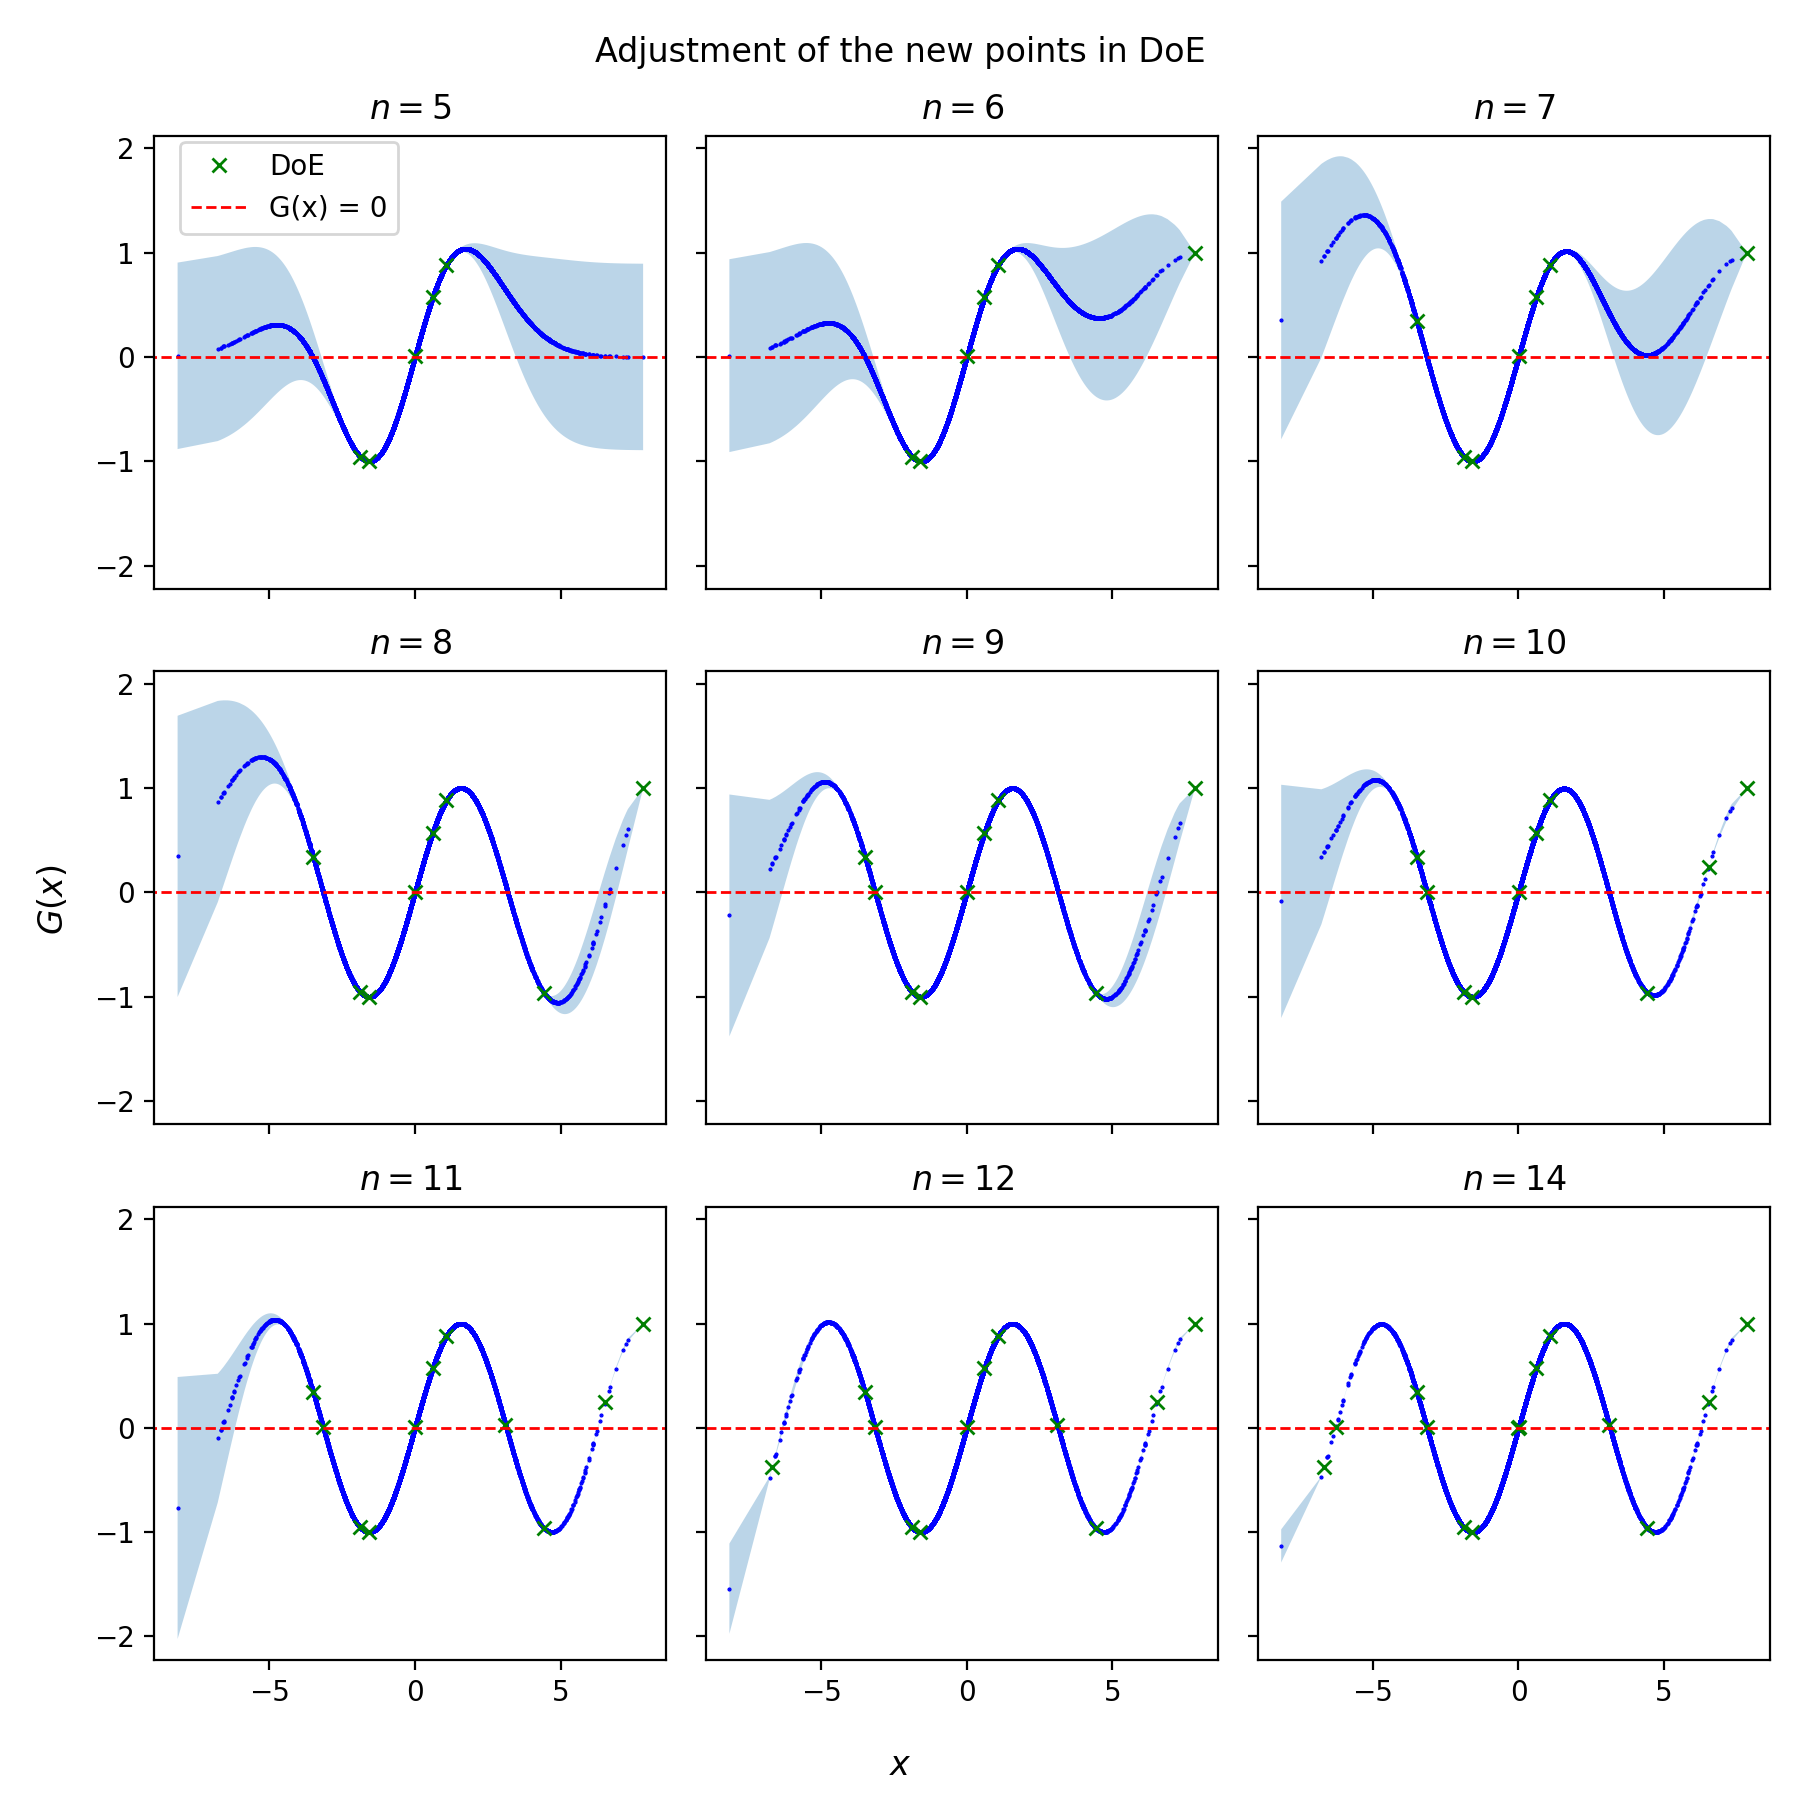
\includegraphics{1d_exa_1d.png}
    \caption{Example 1. Prediction and standard deviation obtained with $n$ points
    in the DoE.}
    \label{fig:ex1}
\end{figure}

\begin{table}[h]
  \footnotesize%
  \begin{center}
  \begin{tabular}{lclcc}
  \toprule
  Method & $N_{call}$  & $\widehat{p_f}$ $(\text{C.O.V}_{\widehat{p_f}})$ &$\epsilon_{\widehat{p_f}}(\%)$  \\
  \midrule
  Monte Carlo   & \num[round-precision=1,round-mode=figures]{10000} & \num{0.4944}($1.01\%$) & - \\
  AK-MCS+U & $14$ & \num{0.4944} & $0$ \\
  \bottomrule
  \end{tabular}
  \end{center}
  \caption{Results of example 1}
  \label{tab:res_ex1}
\end{table}

In figure \ref{fig:ex1} it can be seen how the algorithm selects the next point to
be added to the DoE such that it reduces the most the variance near to the limit 
$G(\pmb{x}) = 0$. Even though there is still some considerable variance in some regions,
it stops at $N = 14$ because this uncertainty is away from the limit, so it is
unlikely to affect the estimation of the probability of failure.
In fact, the results in table \ref{tab:res_ex1} reveal that a very accurate estimation
is obtained.

\subsection{Example 2}
In the second place there is a series system with four branches that is worked in 
\citep{Echard2011}. Both random variables
are standard normal distributed. The performance function is:
\begin{equation}
    G(x_1, x_2) = \text{min}
    \left\lbrace
    \begin{array}{c@{}l}
      3 + 0.1(x_1-x_2)^2 - \frac{(x_1+x_2)}{\sqrt{2}}; \\
      3 + 0.1(x_1-x_2)^2 + \frac{(x_1+x_2)}{\sqrt{2}}; \\
      (x_1-x_2) + \frac{4}{\sqrt{2}}; \\
      (x_2-x_1) + \frac{4}{\sqrt{2}}
    \end{array}
    \right\rbrace
  \end{equation}
with $k$ taking two different values: $6$ and $7$.

From the results on tables \ref{tab:res_ex2} and \ref{tab:res_ex2_2} we can see
that the learning function U obtained the most accurate estimations of $\widehat{p_f}$,
being exactly the same of the MCS. In the case $k=6$, the other two functions performed
well, they only failed at clasifying one point. In the other one, with $k=7$, EFF made some
misclassifications, but the learning function H, although calling the performance function
less times, had an error of $30\%$. \\

\begin{table}[h]
    \footnotesize
    \begin{center}
    \begin{tabular}{lclc}
    \toprule
    Method & $N_{call}$  & $\widehat{p_f}$ $(\text{C.O.V}_{\widehat{p_f}})$ &$\epsilon_{\widehat{p_f}}(\%)$  \\
    \midrule
    Monte Carlo   & \num[round-precision=1,round-mode=figures]{1000000} & \num{0.004433}($1.5\%$) & - \\
    AK-MCS+U & $126$ & \num{0.004433} & $0$ \\
    AK-MCS+EFF & $123$ & \num{0.004432} & $0.02$ \\
    AK-MCS+H & $113$ & \num{0.004434} & $0.02$ \\
    \bottomrule
    \end{tabular}
    \end{center}
    \caption{Results of example 2 with $k=6$}
    \label{tab:res_ex2}
\end{table}

\begin{table}[h]
    \footnotesize
    \begin{center}
    \begin{tabular}{lclc}
    \toprule
    Method & $N_{call}$  & $\widehat{p_f}$ $(\text{C.O.V}_{\widehat{p_f}})$ &$\epsilon_{\widehat{p_f}}(\%)$  \\
    \midrule
    Monte Carlo   & \num[round-precision=1,round-mode=figures]{1000000} & \num{0.002161}($2.15\%$) & - \\
    AK-MCS+U & $103$ & \num{0.002161} & $0$ \\
    AK-MCS+EFF & $107$ & \num{0.002156} & $0.23$ \\
    AK-MCS+H & $65$ & \num{0.0015} & $30.59$ \\
    \bottomrule
    \end{tabular}
    \end{center}
    \caption{Results of example 2 with $k=7$}
    \label{tab:res_ex2_2}
\end{table}

In the figure \ref{fig:ex2_mc} the actual distribution of the two classes in the
MC population is displayed, while in the figure \ref{fig:ex2_iteru} there is the
distribution predicted by AK-MCS+U at several stages. Additionally, figure \ref{fig:ex2_iteru}
give some insights about the update of the DoE, showing how the selected points tend to
come from near the limit $G(\pmb{x}) = 0$. \\

\begin{figure}[h]
    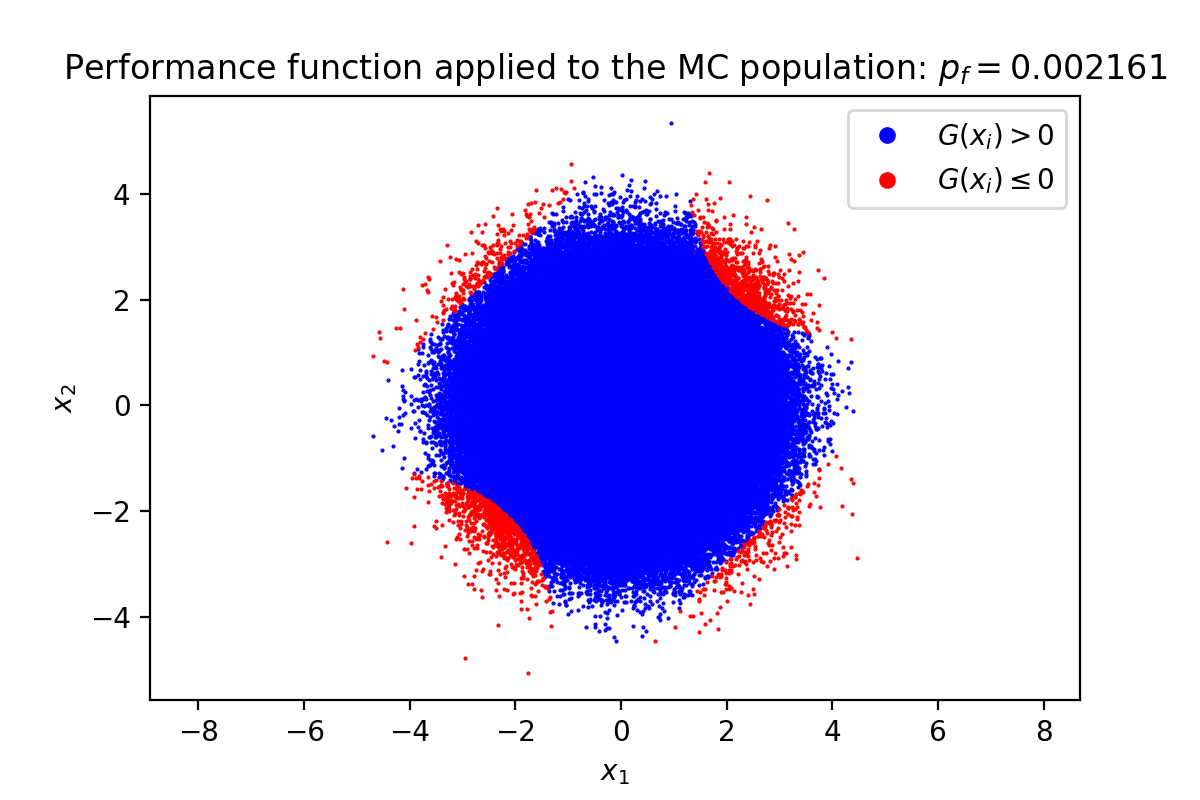
\includegraphics[width=0.8\linewidth]{mc_ex_2D_k7.png}
    \caption{Example 2 with $k=7$. Evaluation of the performance function on the MC population.}
    \label{fig:ex2_mc}
\end{figure}

\begin{figure*}[h]
    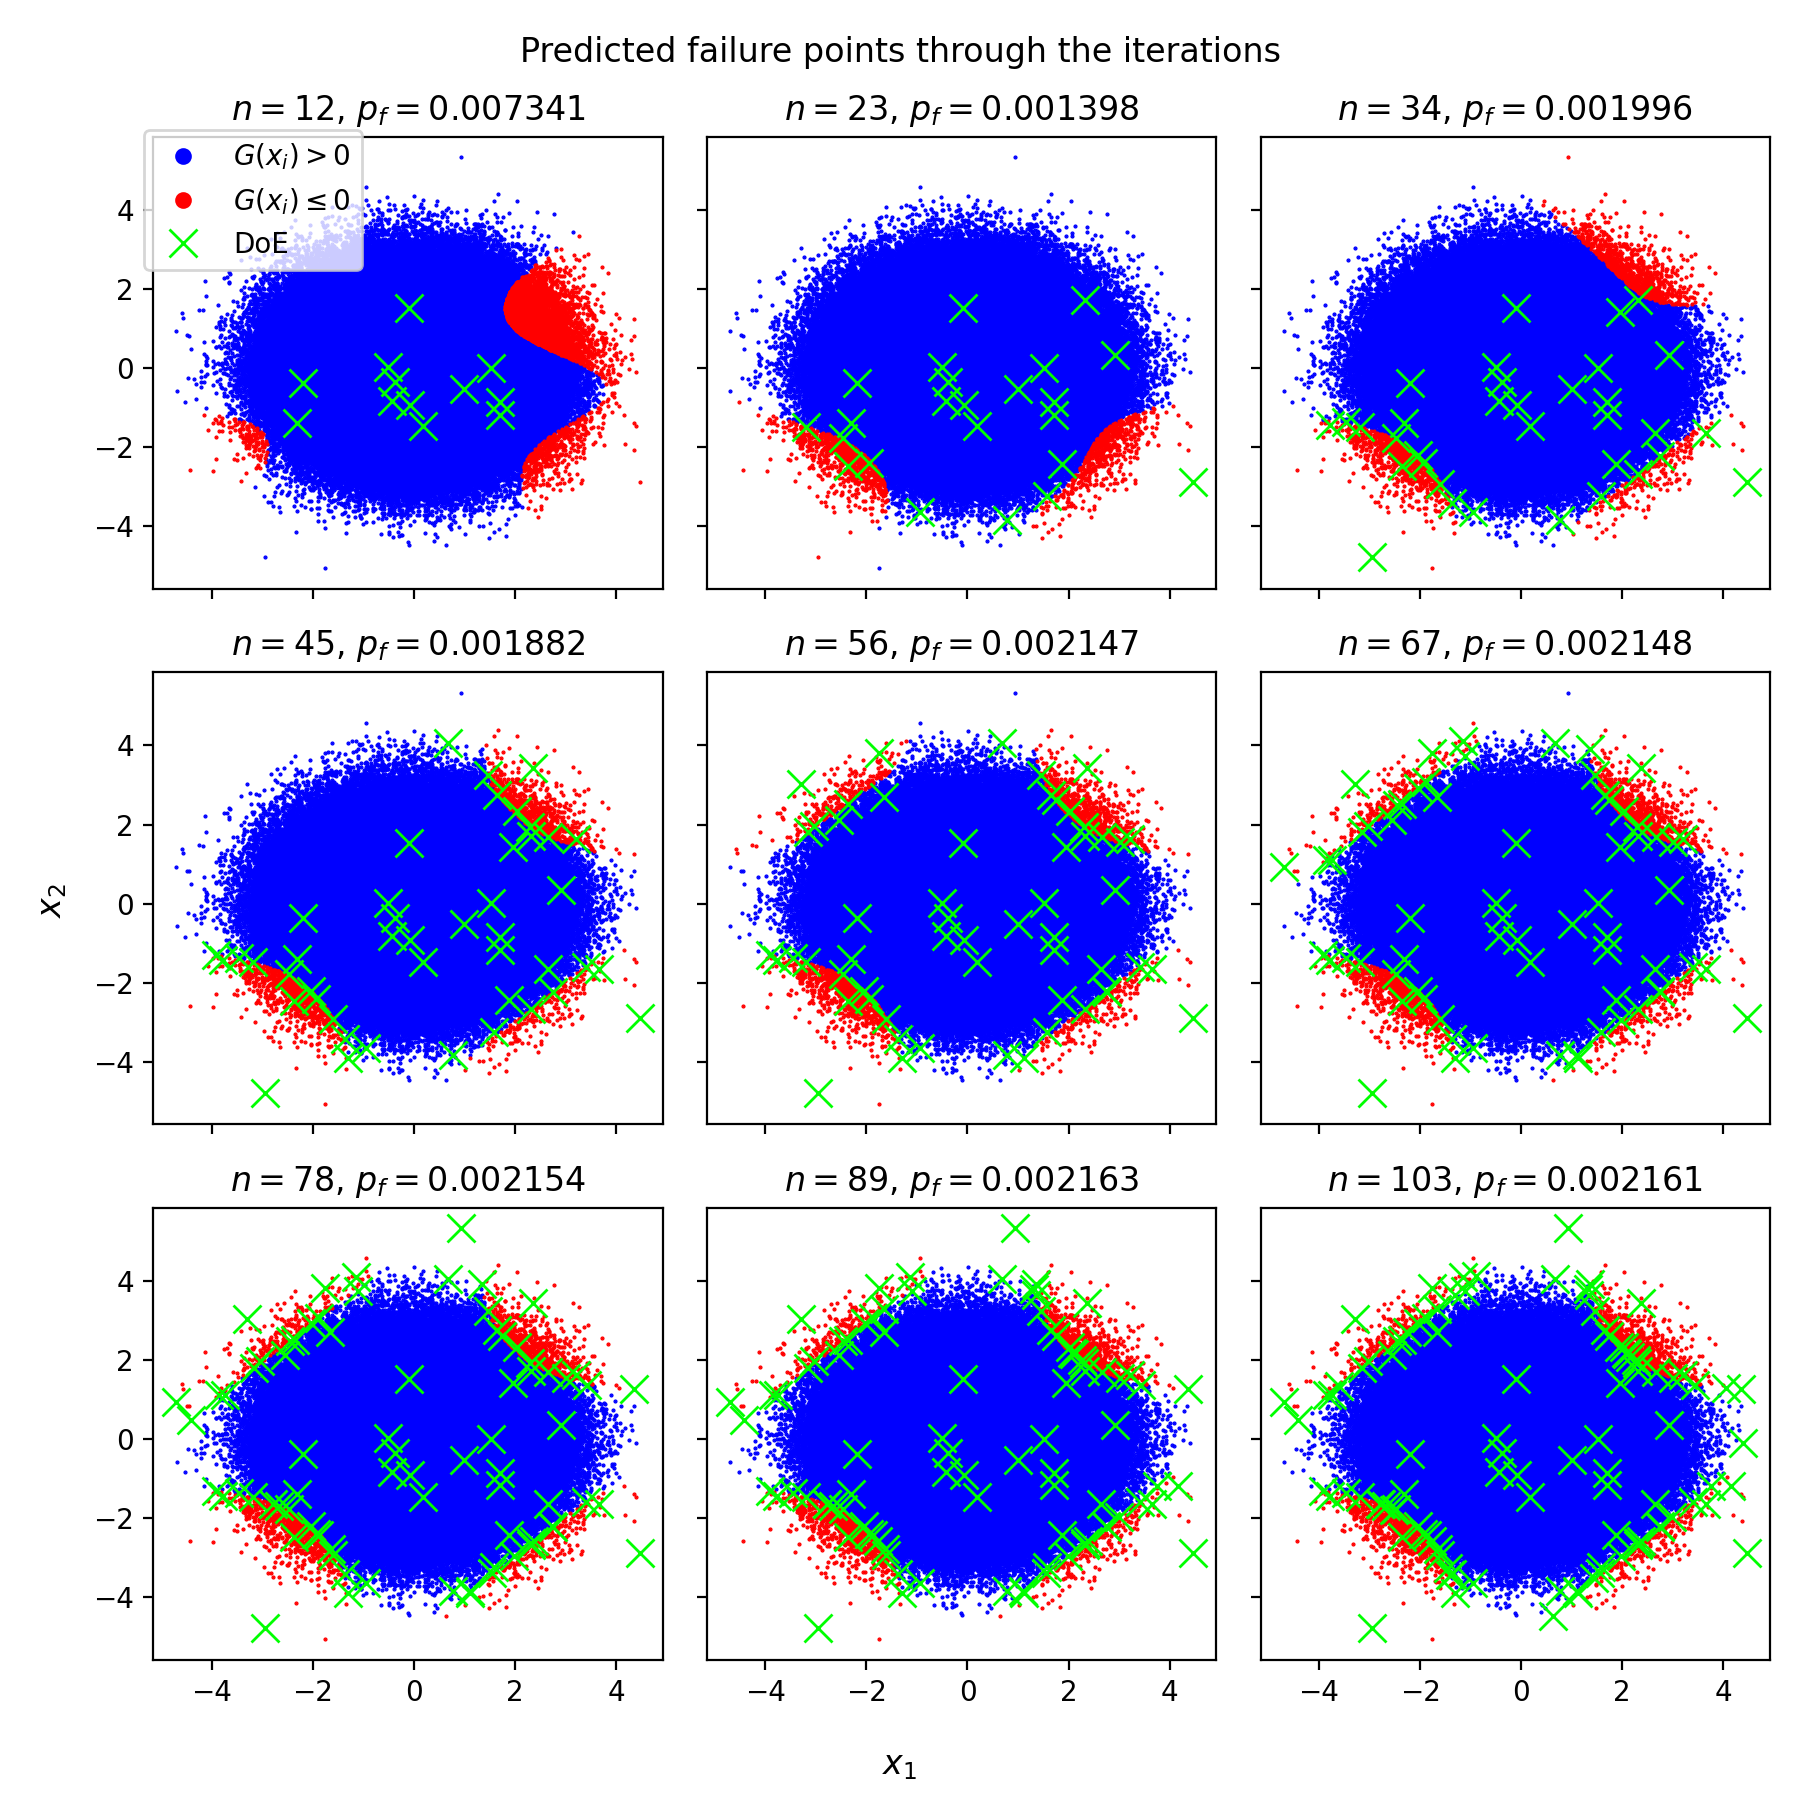
\includegraphics{iter_ex_2D_k7_U.png}
    \caption{Example 2 with $k=7$. Prediction made by AK-MCS+U at several stages.}
    \label{fig:ex2_iteru}
\end{figure*}

Figures  \ref{fig:ex2_k6} and \ref{fig:ex2_k7} display how the probability of failure
converges with each learning function, and how the selected points make the learning criteria
tend to the stopping conditions. In both cases there are similar behaviors. The 
EFF is proned to converge more consistently to the stopping condition. The function 
U usually gets a good estimation well before finishing. The function H
presents the most irregular results. A stricter stopping condition would be more appropiate
for this last learning function.

\begin{figure*}[h]
    \begin{subfigure}{.5\textwidth}
        \centering
        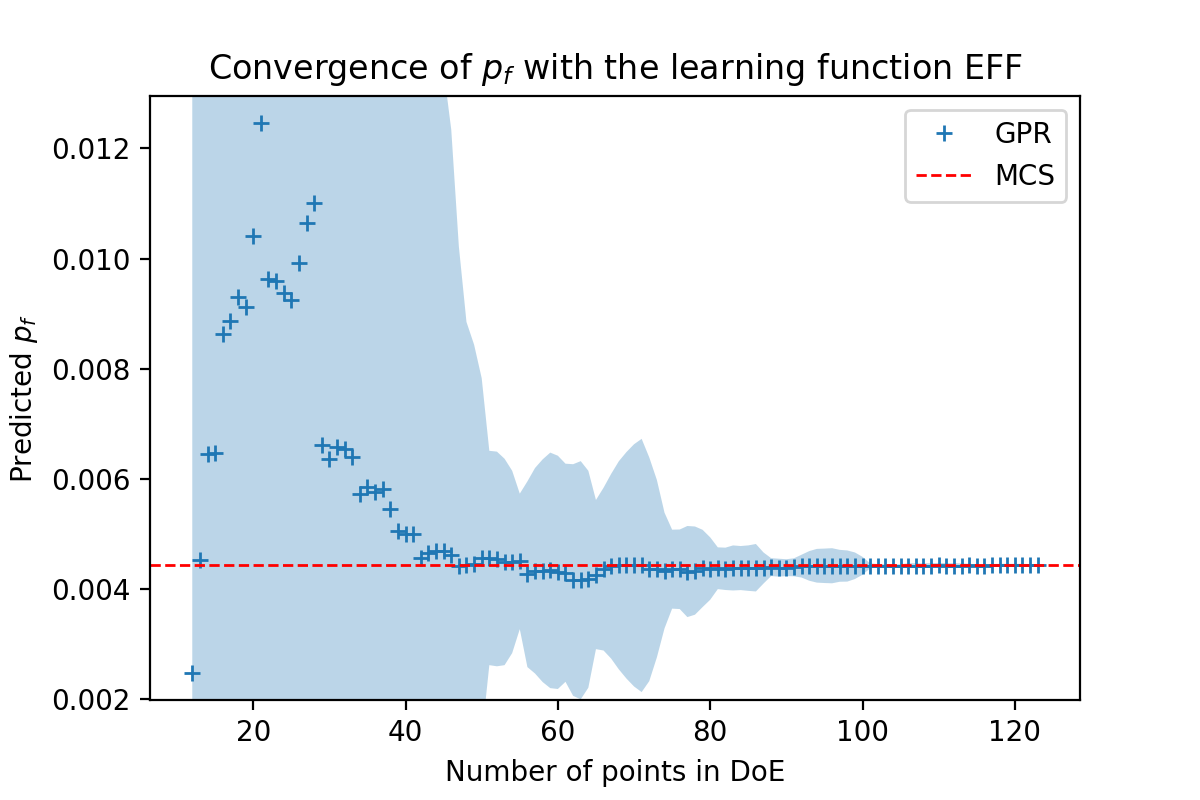
\includegraphics[width=\linewidth]{conv_ex_2D_k6_EFF.png}
      \end{subfigure}%
      \begin{subfigure}{.5\textwidth}
        \centering
        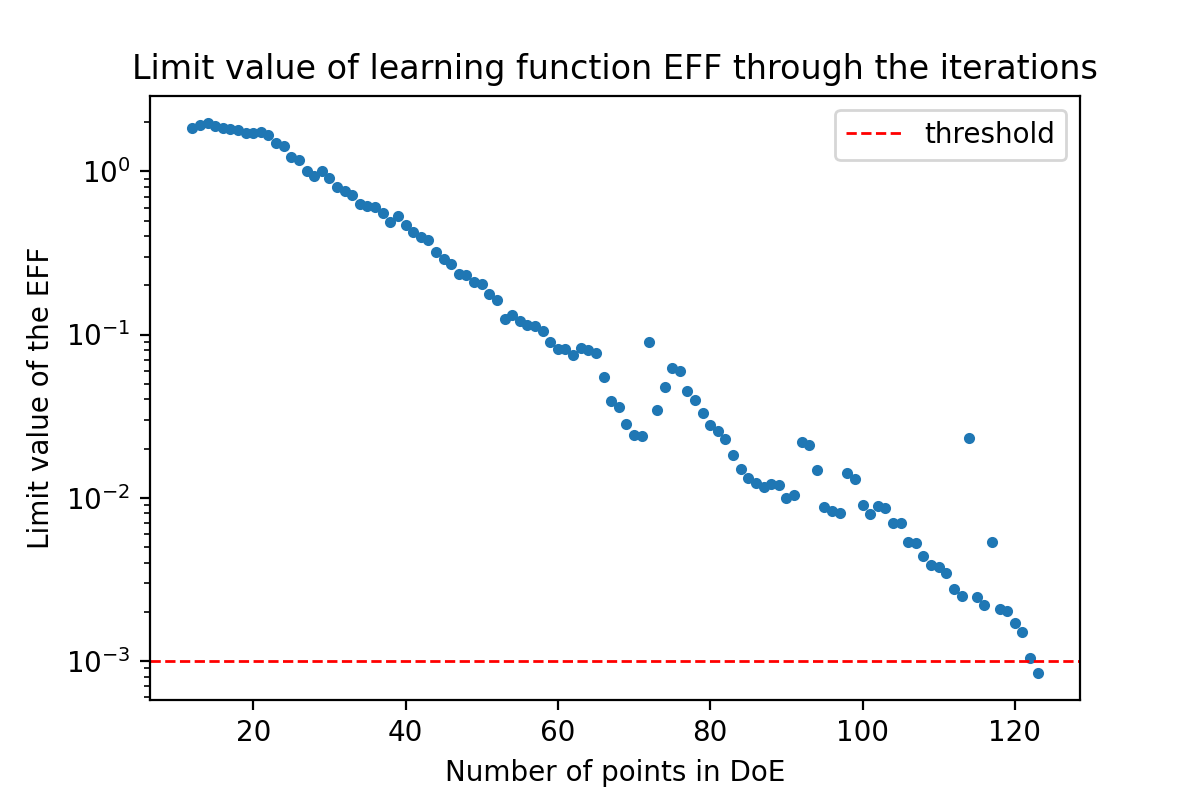
\includegraphics[width=\linewidth]{ex_2D_k6_EFF_lim_values.png}
      \end{subfigure}%
      \\
      \begin{subfigure}{.5\textwidth}
        \centering
        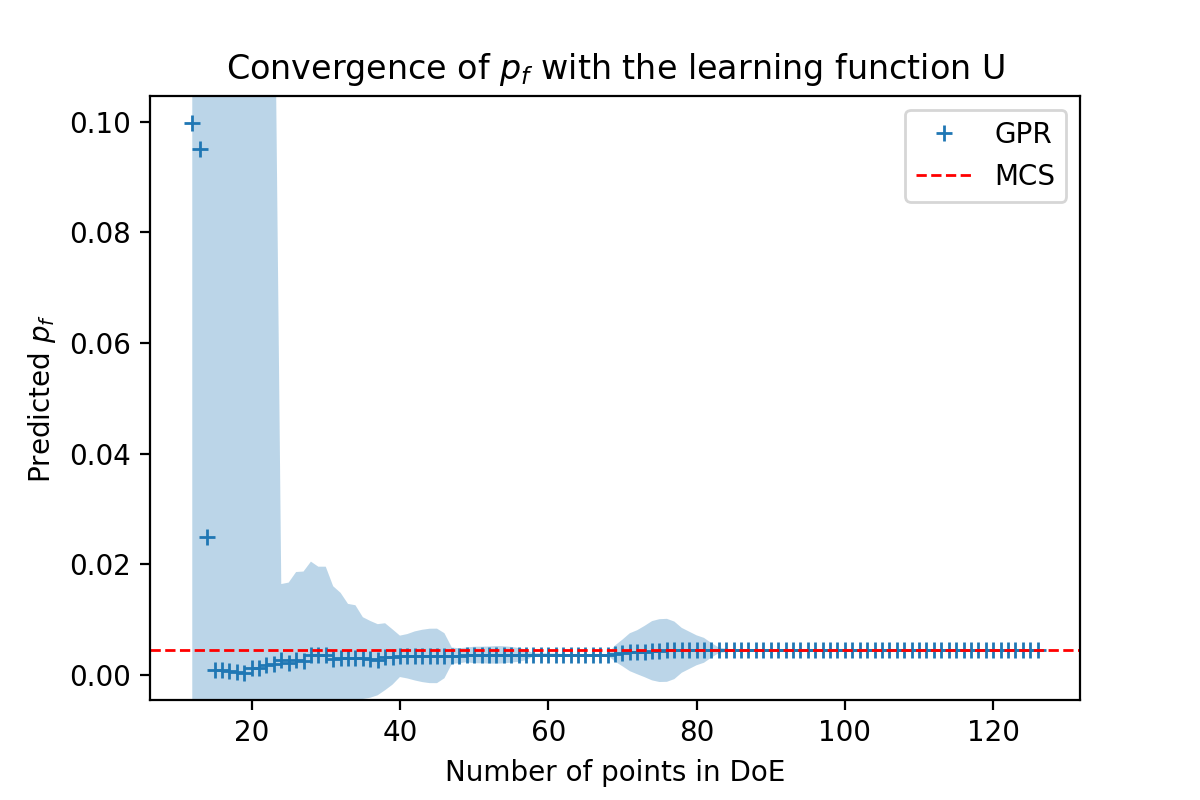
\includegraphics[width=\linewidth]{conv_ex_2D_k6_U.png}
      \end{subfigure}%
      \begin{subfigure}{.5\textwidth}
        \centering
        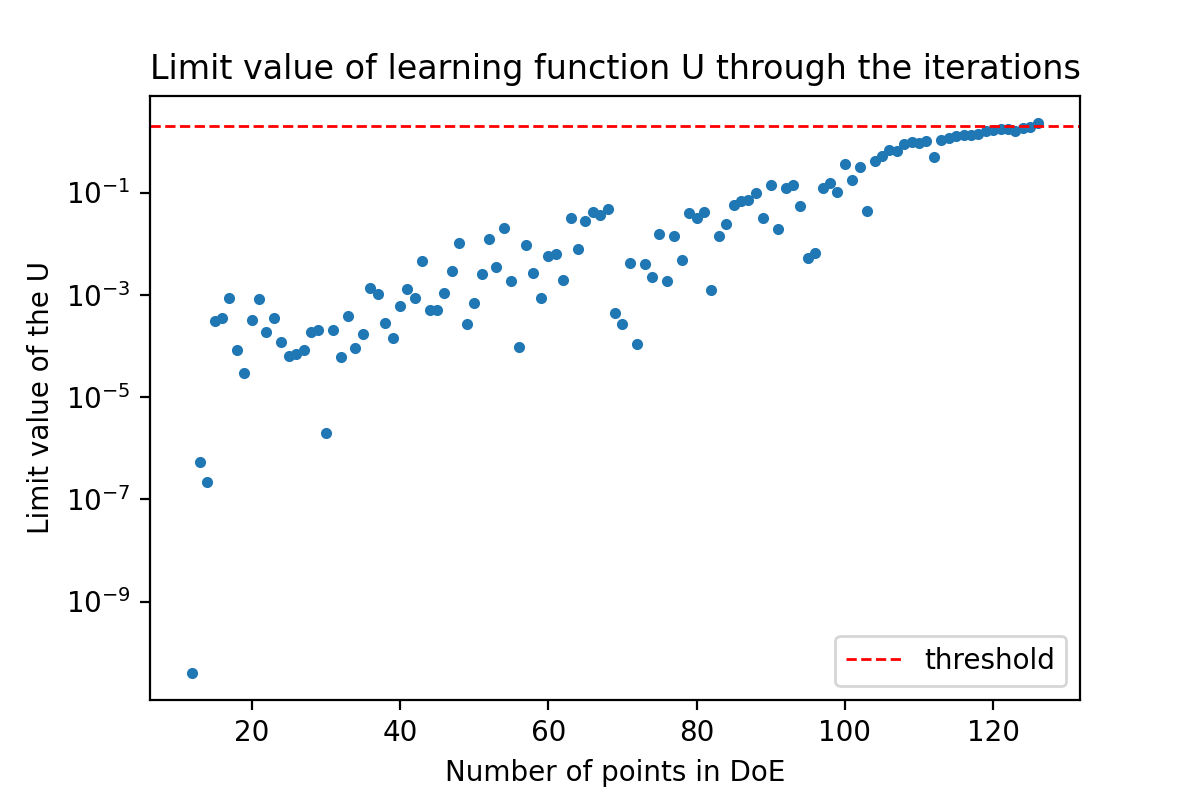
\includegraphics[width=\linewidth]{ex_2D_k6_U_lim_values.png}
      \end{subfigure}%
      \\    \begin{subfigure}{.5\textwidth}
        \centering
        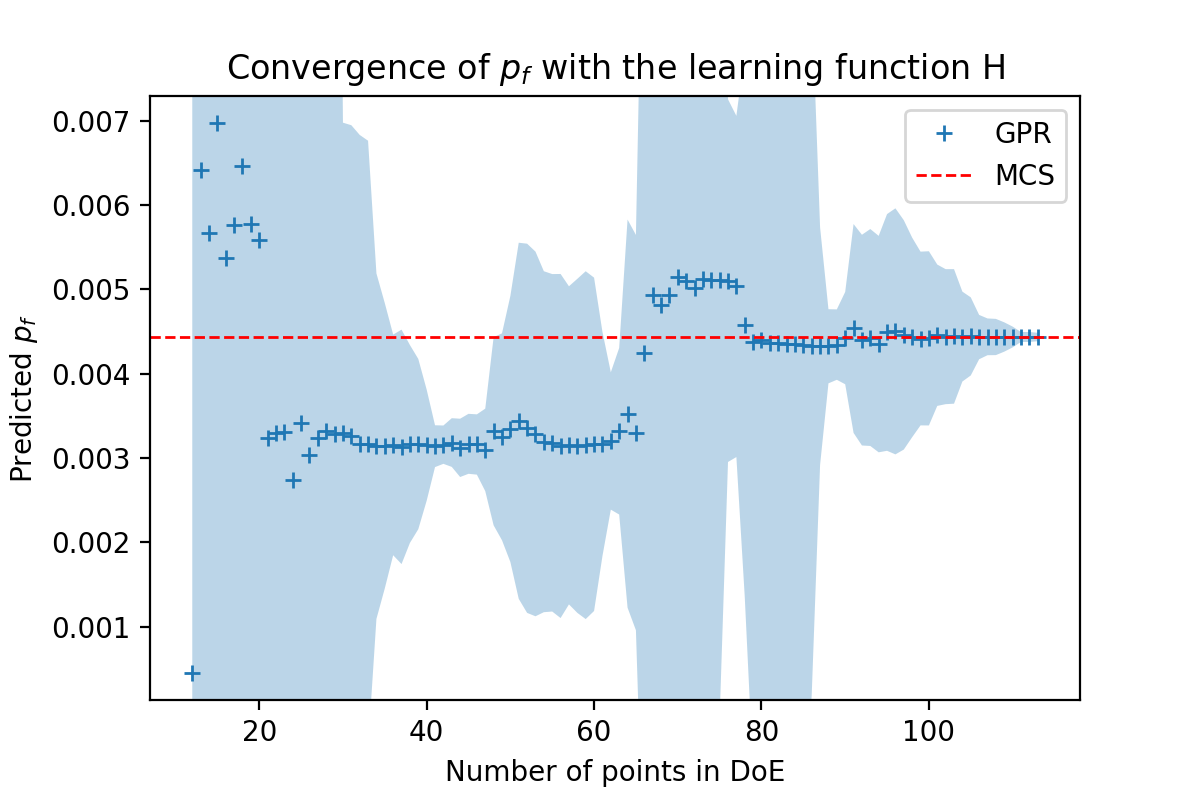
\includegraphics[width=\linewidth]{conv_ex_2D_k6_H.png}
      \end{subfigure}%
      \begin{subfigure}{.5\textwidth}
        \centering
        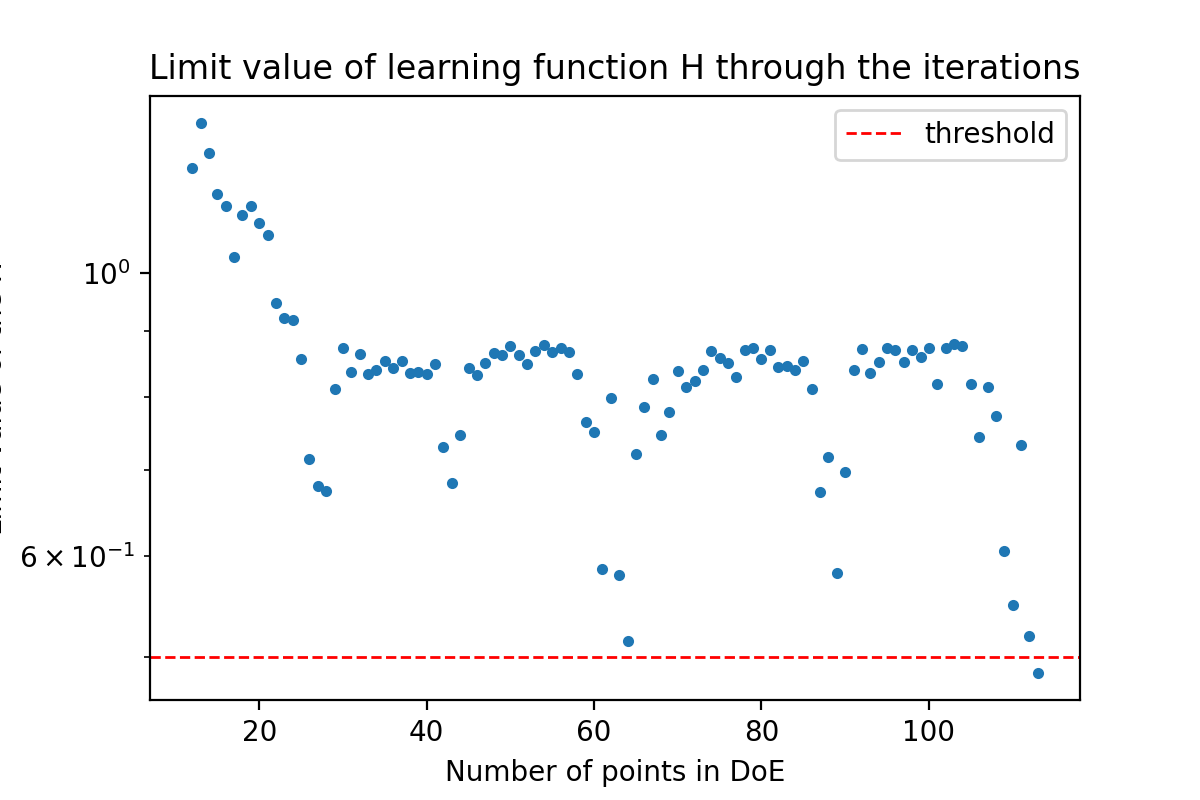
\includegraphics[width=\linewidth]{ex_2D_k6_H_lim_values.png}
      \end{subfigure}%
      \caption{Results of example 2 with $k=6$}
      \label{fig:ex2_k6}
\end{figure*}

\begin{figure*}[h]
    \begin{subfigure}{.5\textwidth}
        \centering
        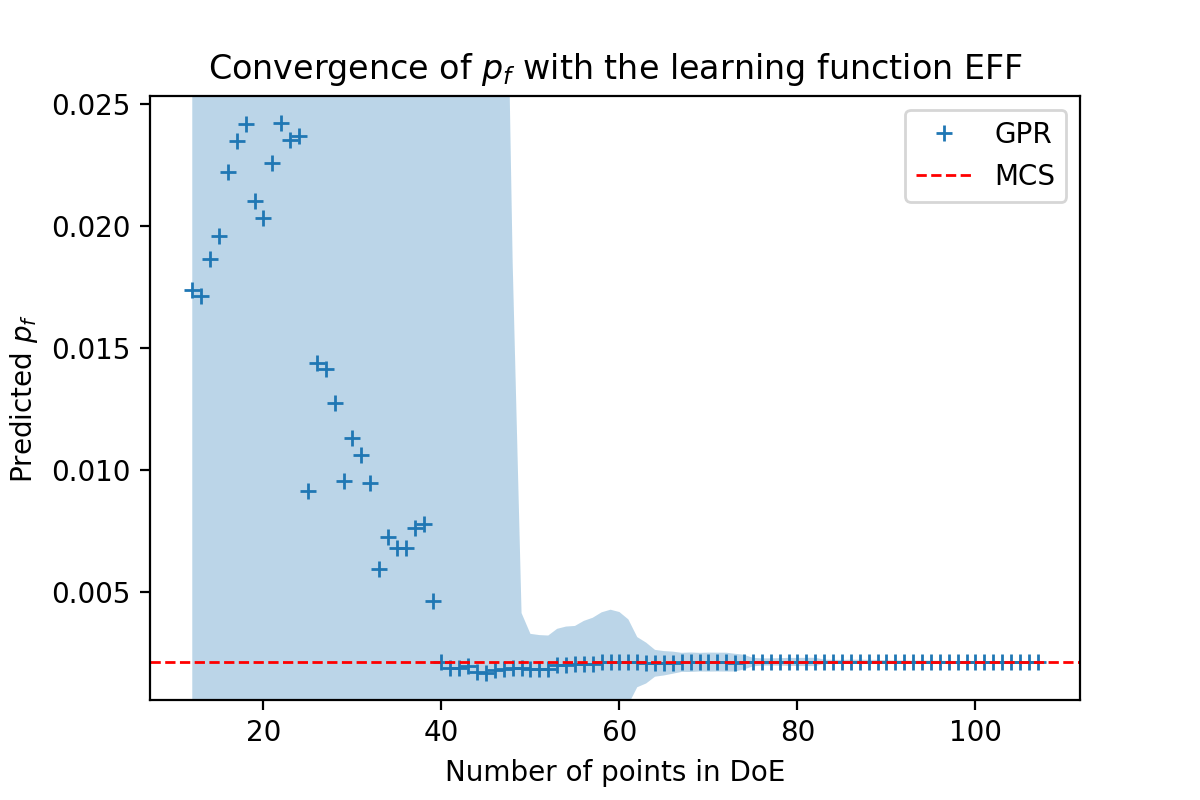
\includegraphics[width=\linewidth]{conv_ex_2D_k7_EFF.png}
      \end{subfigure}%
      \begin{subfigure}{.5\textwidth}
        \centering
        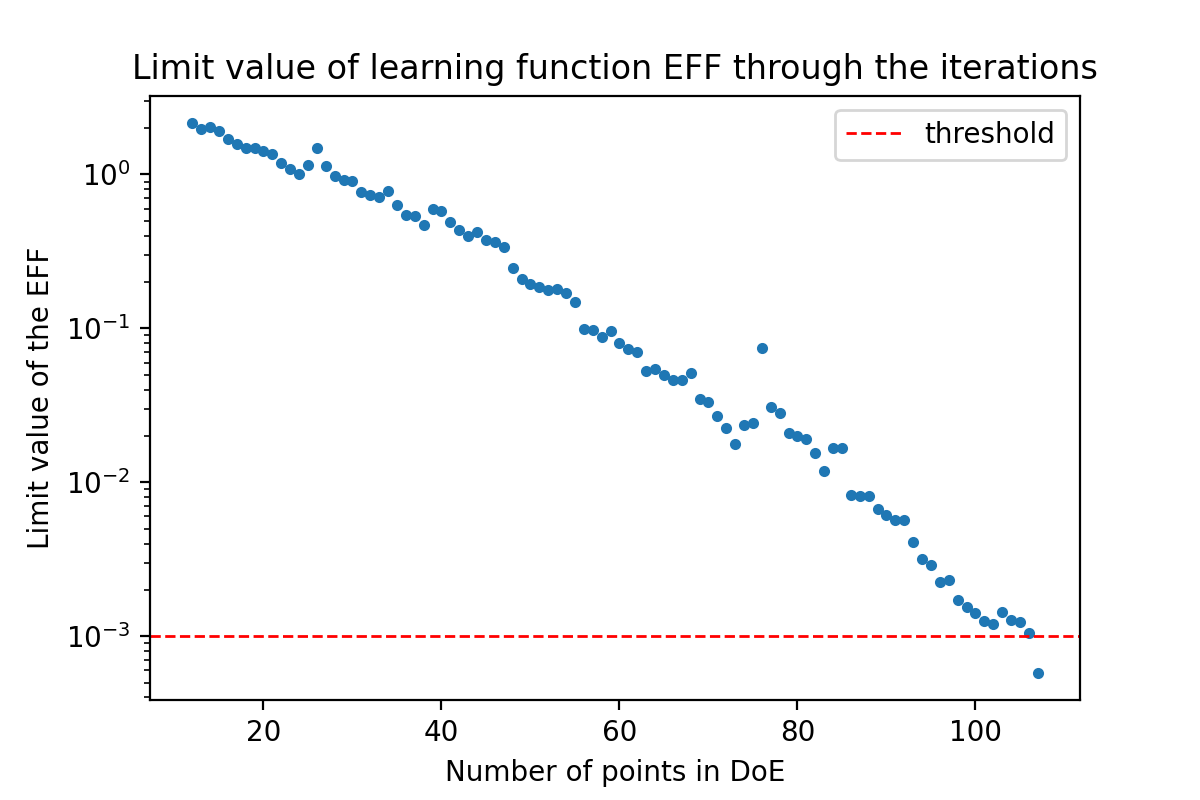
\includegraphics[width=\linewidth]{ex_2D_k7_EFF_lim_values.png}
      \end{subfigure}%
      \\
      \begin{subfigure}{.5\textwidth}
        \centering
        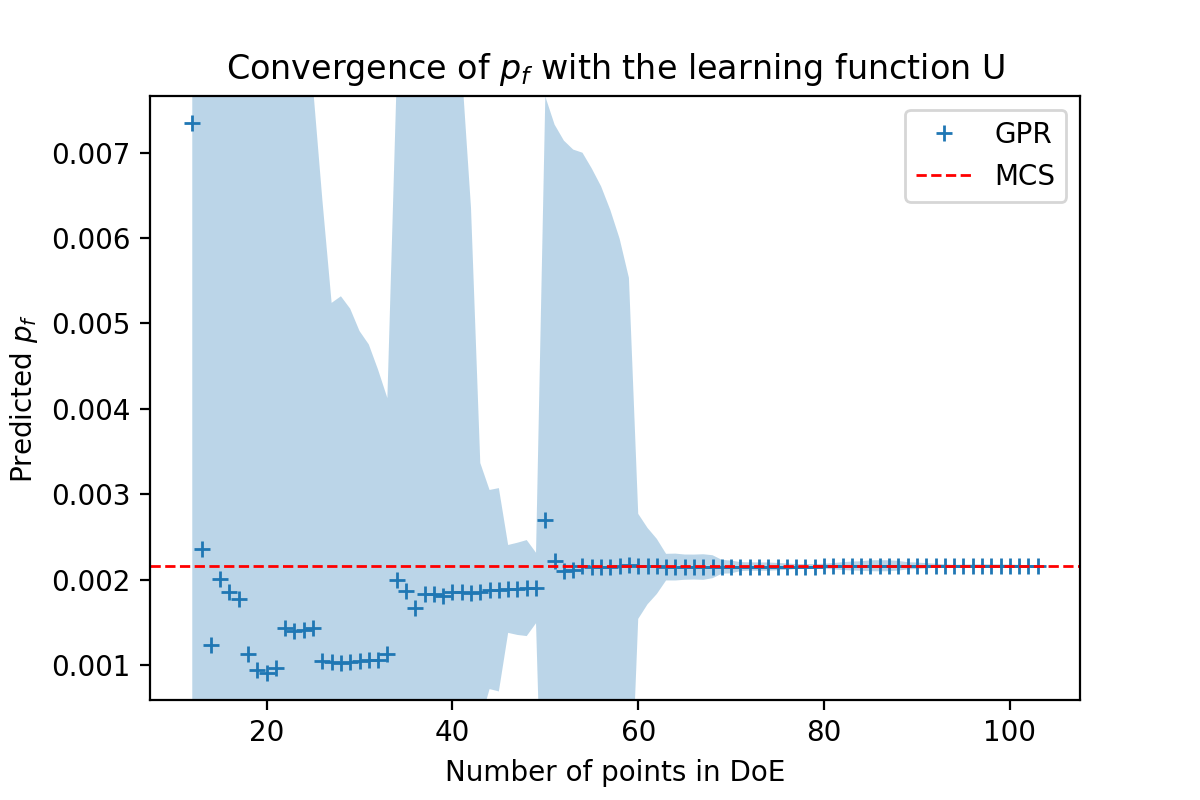
\includegraphics[width=\linewidth]{conv_ex_2D_k7_U.png}
      \end{subfigure}%
      \begin{subfigure}{.5\textwidth}
        \centering
        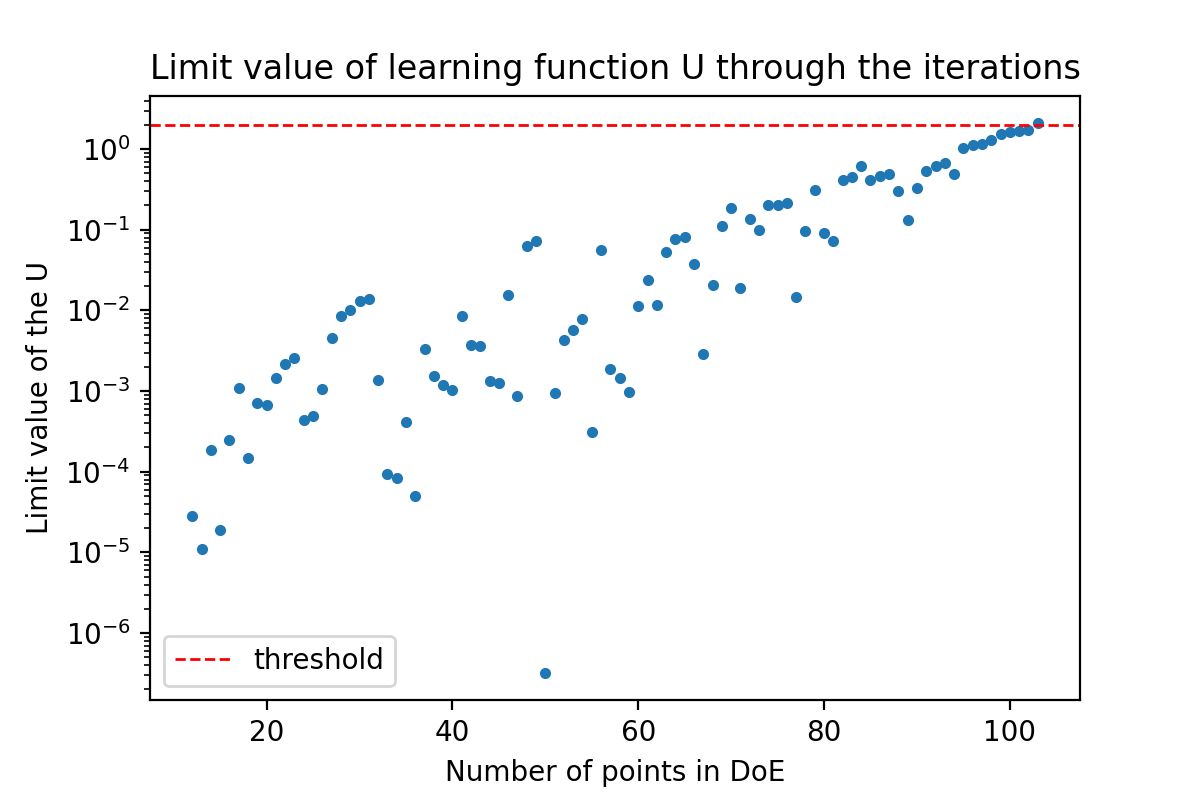
\includegraphics[width=\linewidth]{ex_2D_k7_U_lim_values.png}
      \end{subfigure}%
      \\    \begin{subfigure}{.5\textwidth}
        \centering
        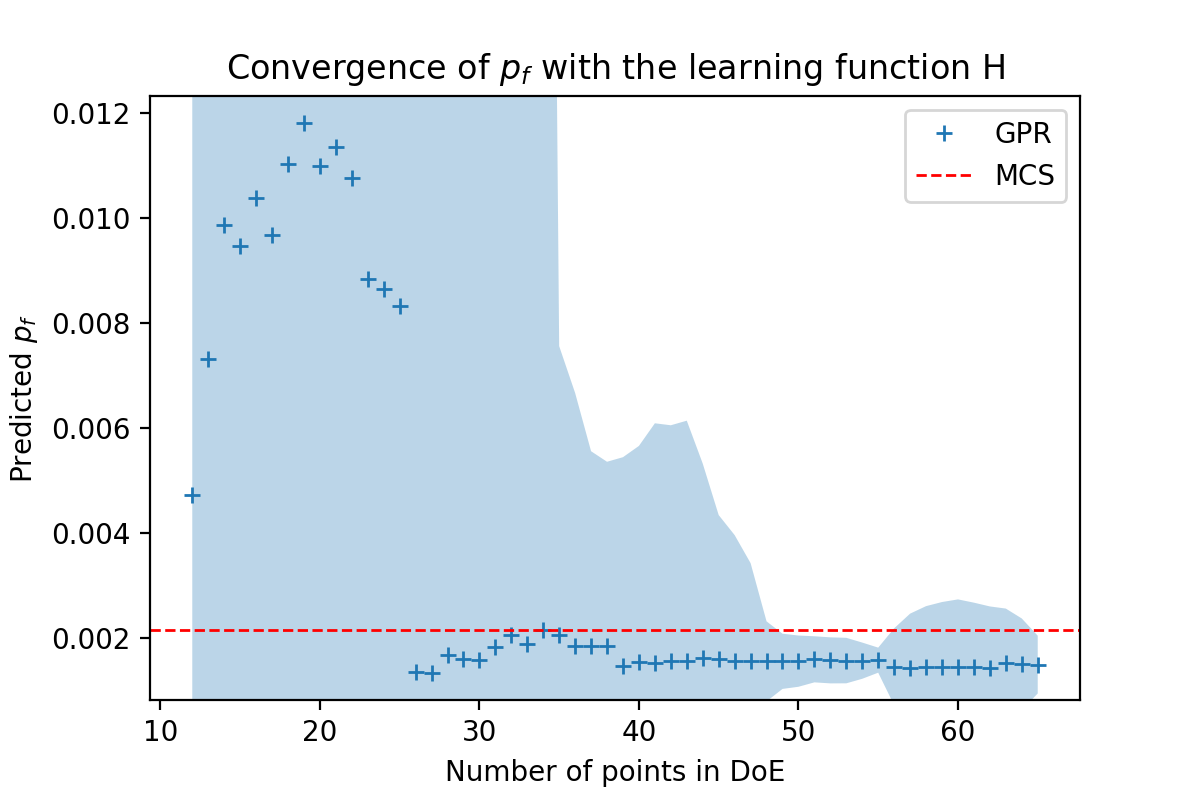
\includegraphics[width=\linewidth]{conv_ex_2D_k7_H.png}
      \end{subfigure}%
      \begin{subfigure}{.5\textwidth}
        \centering
        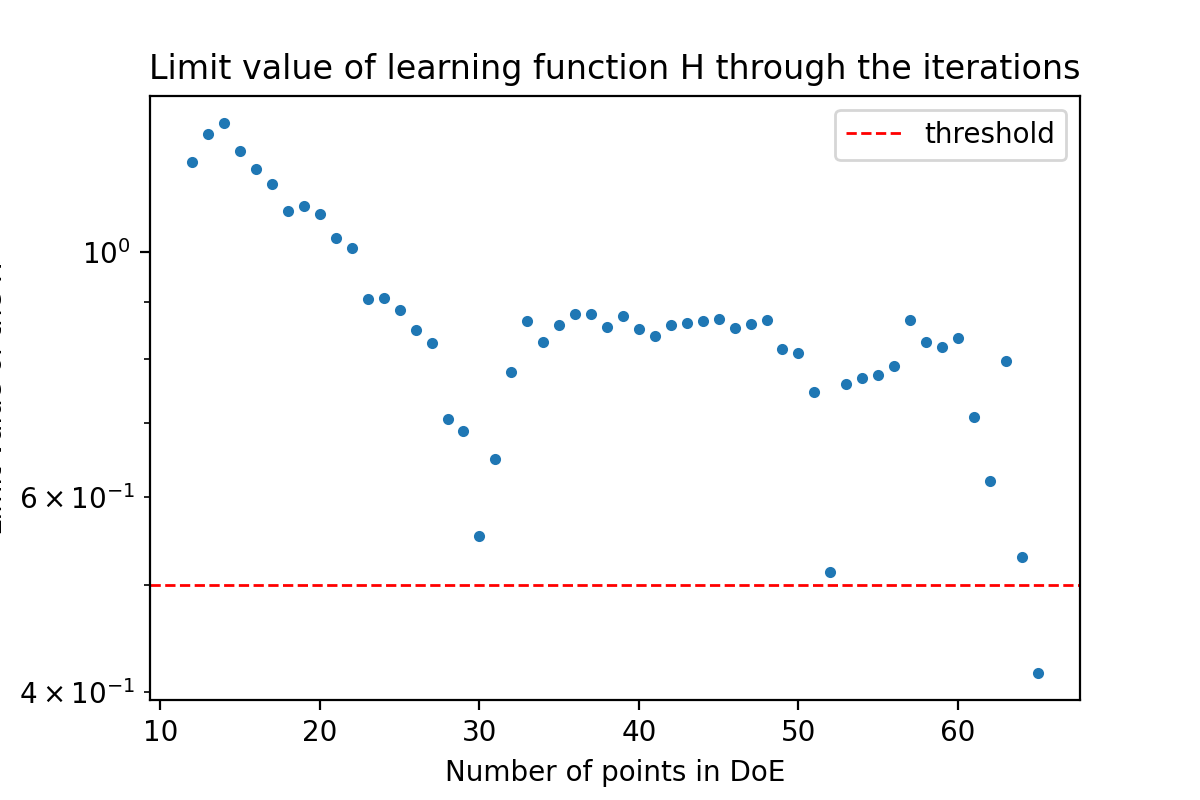
\includegraphics[width=\linewidth]{ex_2D_k7_H_lim_values.png}
      \end{subfigure}%
      \caption{Results of example 2 with $k=7$}
      \label{fig:ex2_k7}
\end{figure*}

\newpage
\subsection{Example 3}
The next example is a non-linear undamped single degree of freedom system, as the
one shown in figure \ref{fig:ex3}. The involved variables are listed in table \ref{tab:var_ex3}.

\begin{equation}
  G(\pmb{x}) = 3r - \left\lvert\frac{2F_i}{m\omega_0^2} \sin{\paren{\frac{\omega_0 t_1}{2}}} \right\rvert
\end{equation}
where $\omega_0 = \sqrt{\frac{c_1 + c_2}{m}}$

\begin{figure}[h]
    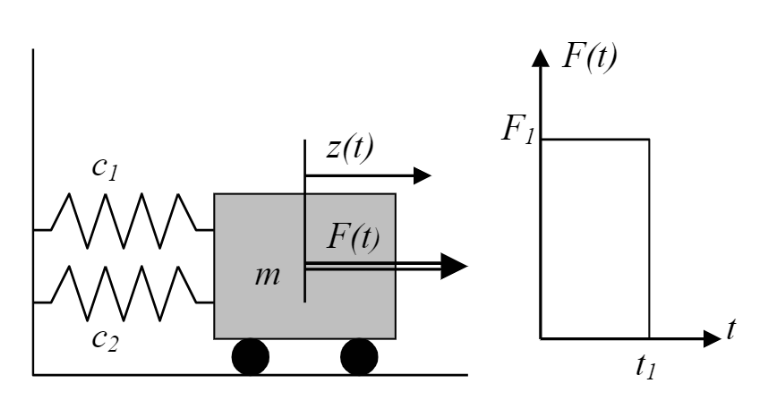
\includegraphics{ex_3.png}
    \caption{Example 3. Non-linear oscilator. Taken from \citep{Schu2005}}
    \label{fig:ex3}
\end{figure}

\begin{table}[h]
    \footnotesize%
    \begin{center}
    \begin{tabular}{cccc}
    \toprule
    Variable & P.D.F & Mean & Standard deviation \\
    \midrule
    $m$   & Normal & $1$ & $0.05$ \\
    $c_1$   & Normal & $1$ & $0.1$ \\
    $c_2$   & Normal & $0.1$ & $0.01$ \\
    $r$   & Normal & $0.5$ & $0.05$ \\
    $F_1$   & Normal & $1$ & $0.2$ \\
    $t_1$   & Normal & $1$ & $0.2$ \\
    \bottomrule
    \end{tabular}
    \end{center}
    \caption{Random variables of example 3}
    \label{tab:var_ex3}
\end{table}

Table \ref{tab:res_ex3} contains the obtained results. In contrast with the other
examples, in this case the function H performs quite well, obtaining the exact result, just
as the function U, but with some more calls to the performance function. \\

In figure \ref{fig:ex3_results} it is evident that the function EFF met its stopping
condition before converging to the solution, unlike the other two functions.

\begin{table}[h]
    \footnotesize
    \begin{center}
    \begin{tabular}{lclc}
    \toprule
    Method & $N_{call}$  & $\widehat{p_f}$ $(\text{C.O.V}_{\widehat{p_f}})$ &$\epsilon_{\widehat{p_f}}(\%)$  \\
    \midrule
    Monte Carlo   & \num[round-precision=1,round-mode=figures]{70000} & \num{0.027814}($2.23\%$) & - \\
    AK-MCS+U & $60$ & \num{0.027814} & $0$ \\
    AK-MCS+EFF & $43$ & \num{0.027671} & $0.51$ \\
    AK-MCS+H & $66$ & \num{0.027814} & $0$ \\
    \bottomrule
    \end{tabular}
    \end{center}
    \caption{Results of example 3}
    \label{tab:res_ex3}
\end{table}

\begin{figure*}[h]
    \begin{subfigure}{.5\textwidth}
        \centering
        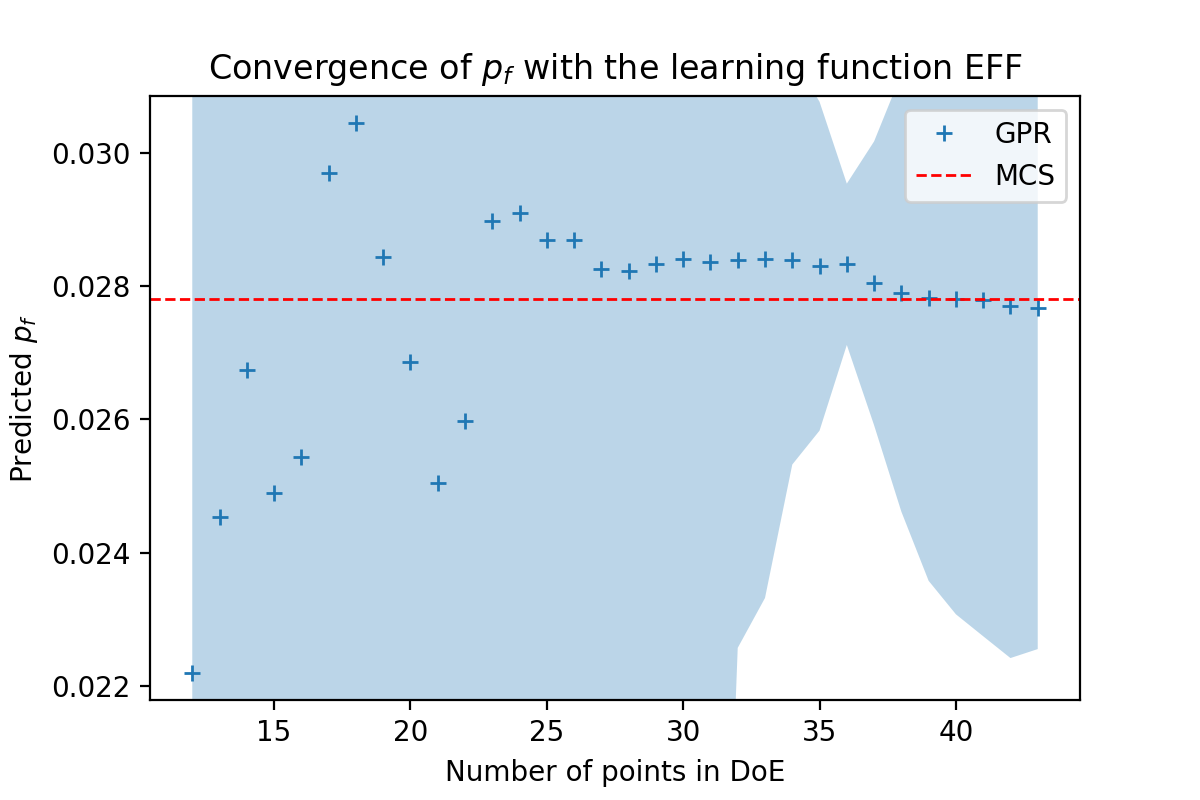
\includegraphics[width=\linewidth]{conv_ex_3_EFF.png}
      \end{subfigure}%
      \begin{subfigure}{.5\textwidth}
        \centering
        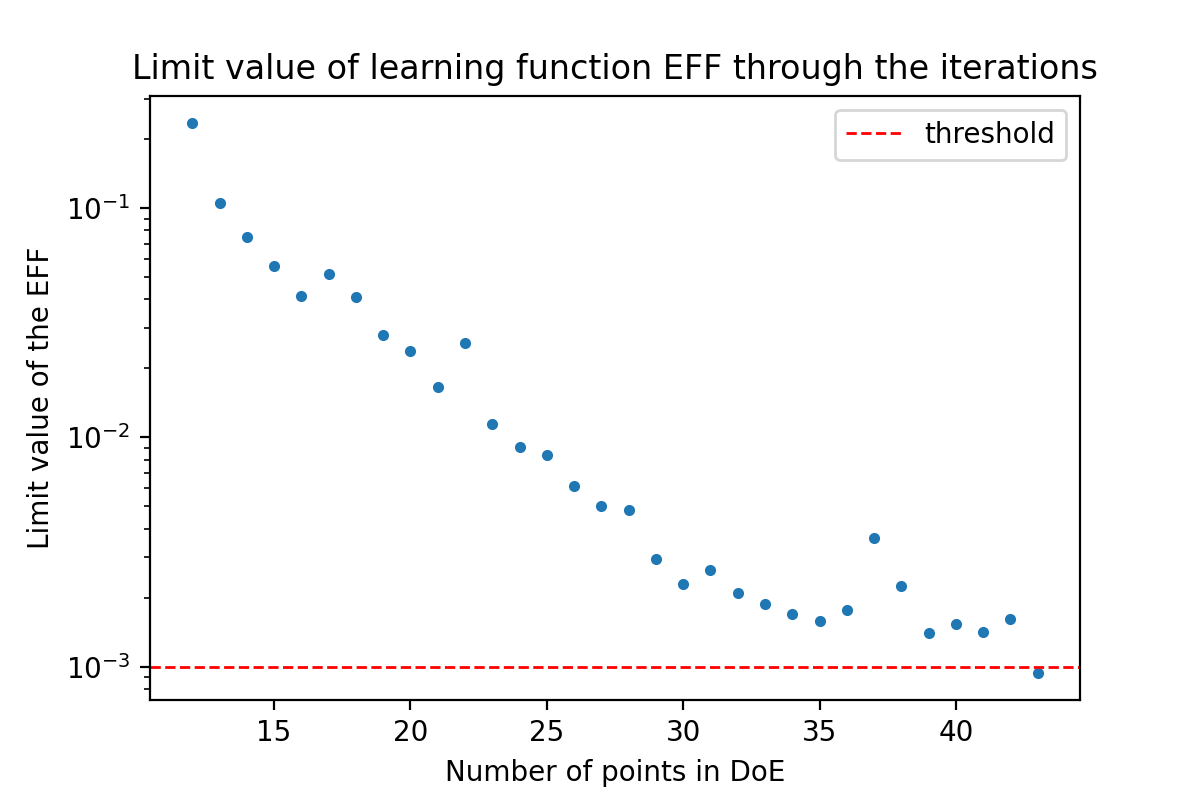
\includegraphics[width=\linewidth]{ex_3_EFF_lim_values.png}
      \end{subfigure}%
      \\
      \begin{subfigure}{.5\textwidth}
        \centering
        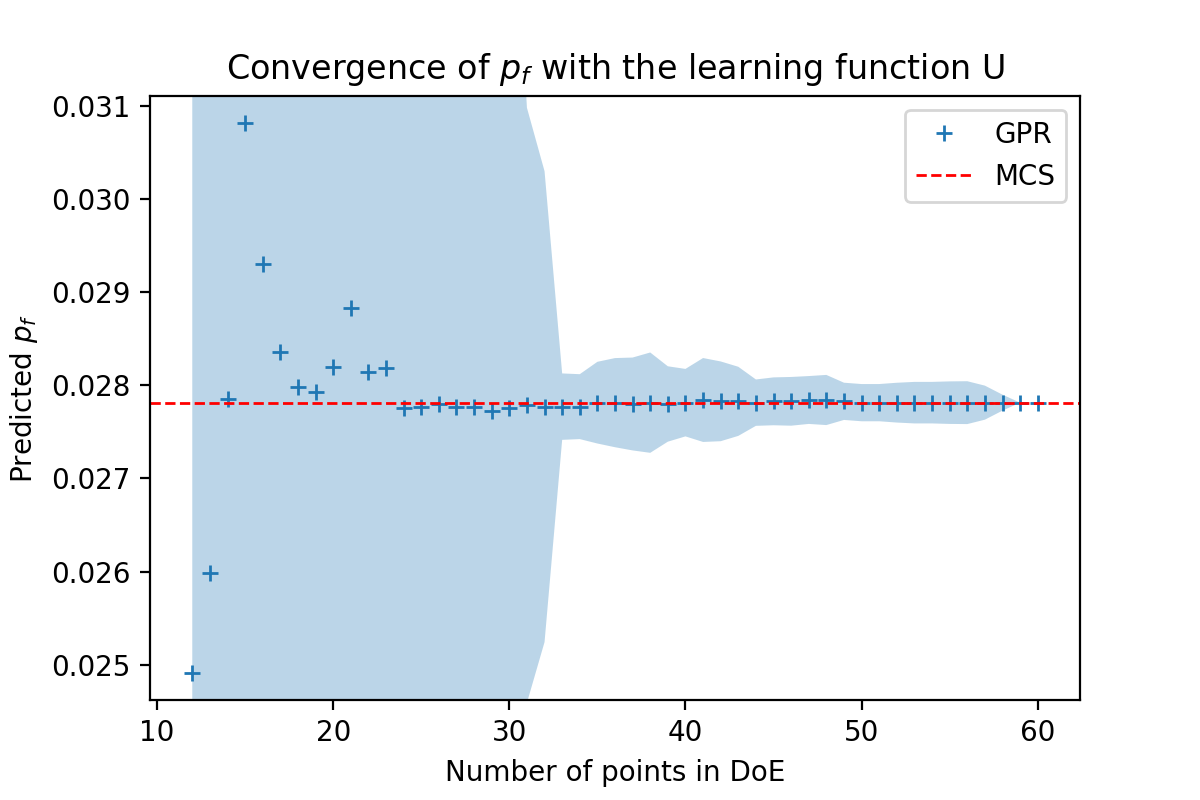
\includegraphics[width=\linewidth]{conv_ex_3_U.png}
      \end{subfigure}%
      \begin{subfigure}{.5\textwidth}
        \centering
        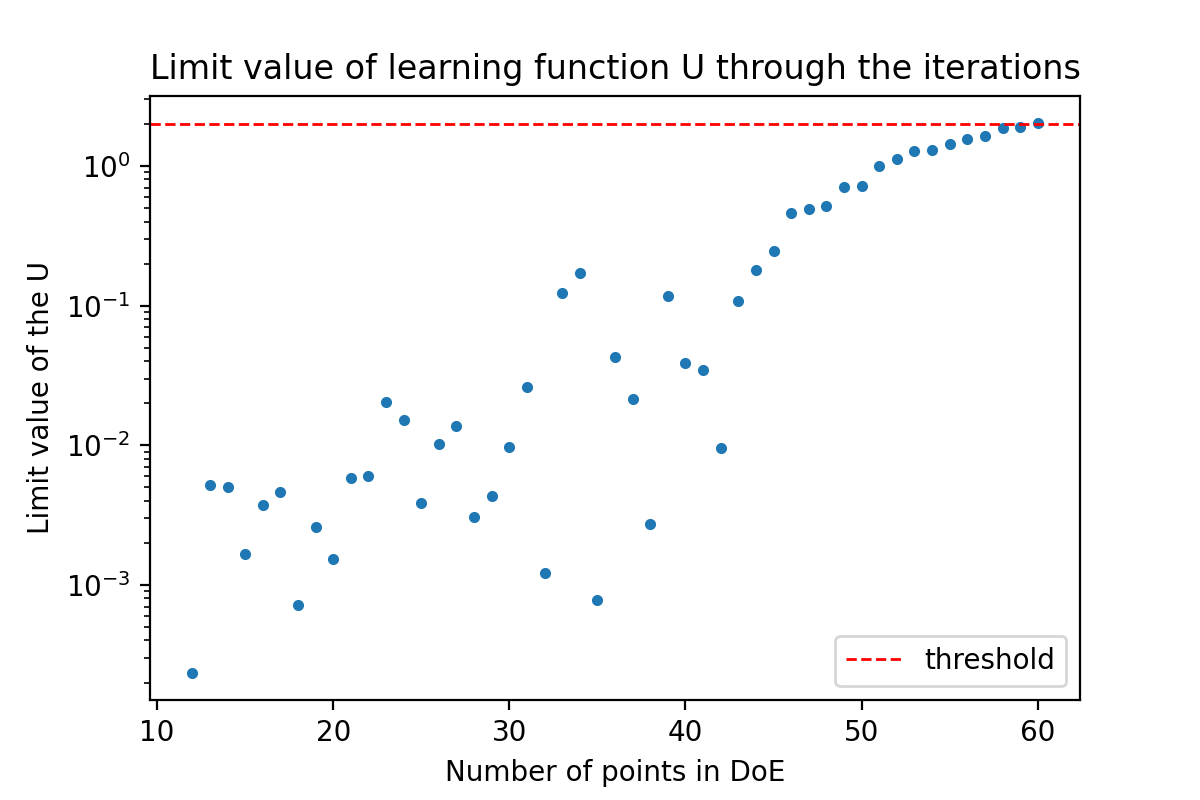
\includegraphics[width=\linewidth]{ex_3_U_lim_values.png}
      \end{subfigure}%
      \\    \begin{subfigure}{.5\textwidth}
        \centering
        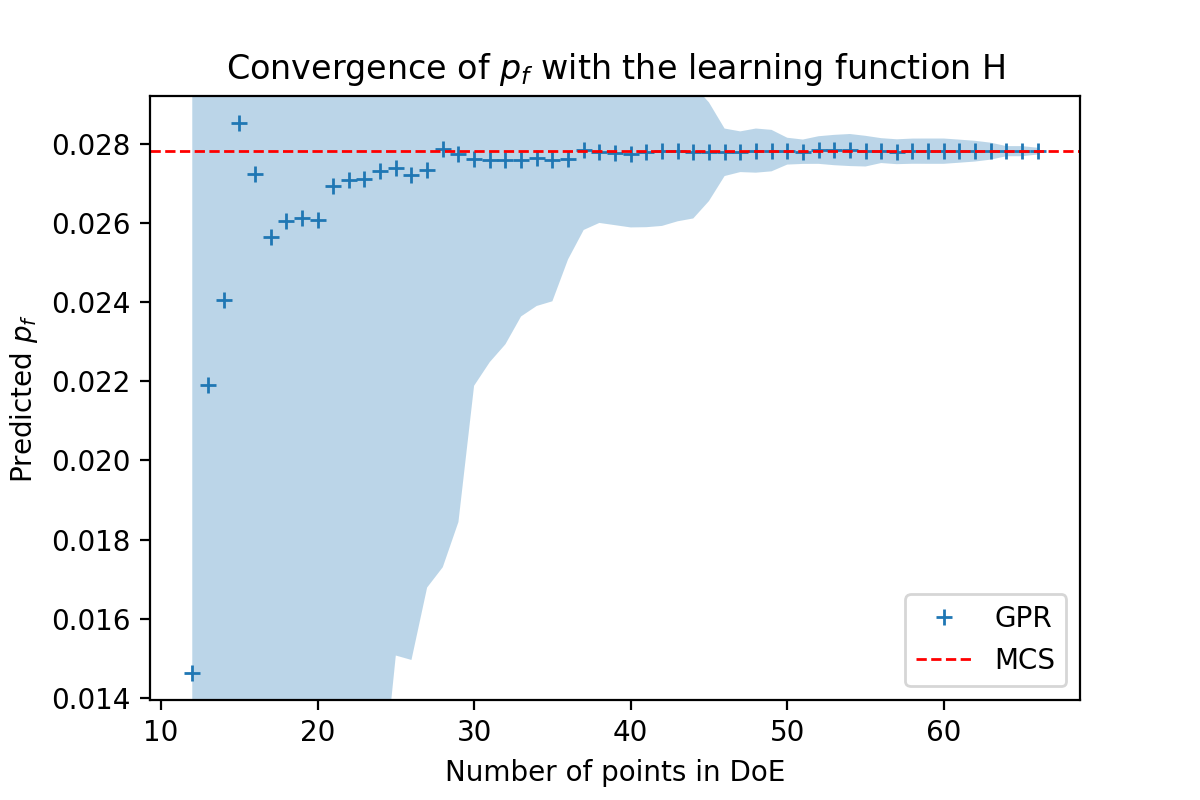
\includegraphics[width=\linewidth]{conv_ex_3_H.png}
      \end{subfigure}%
      \begin{subfigure}{.5\textwidth}
        \centering
        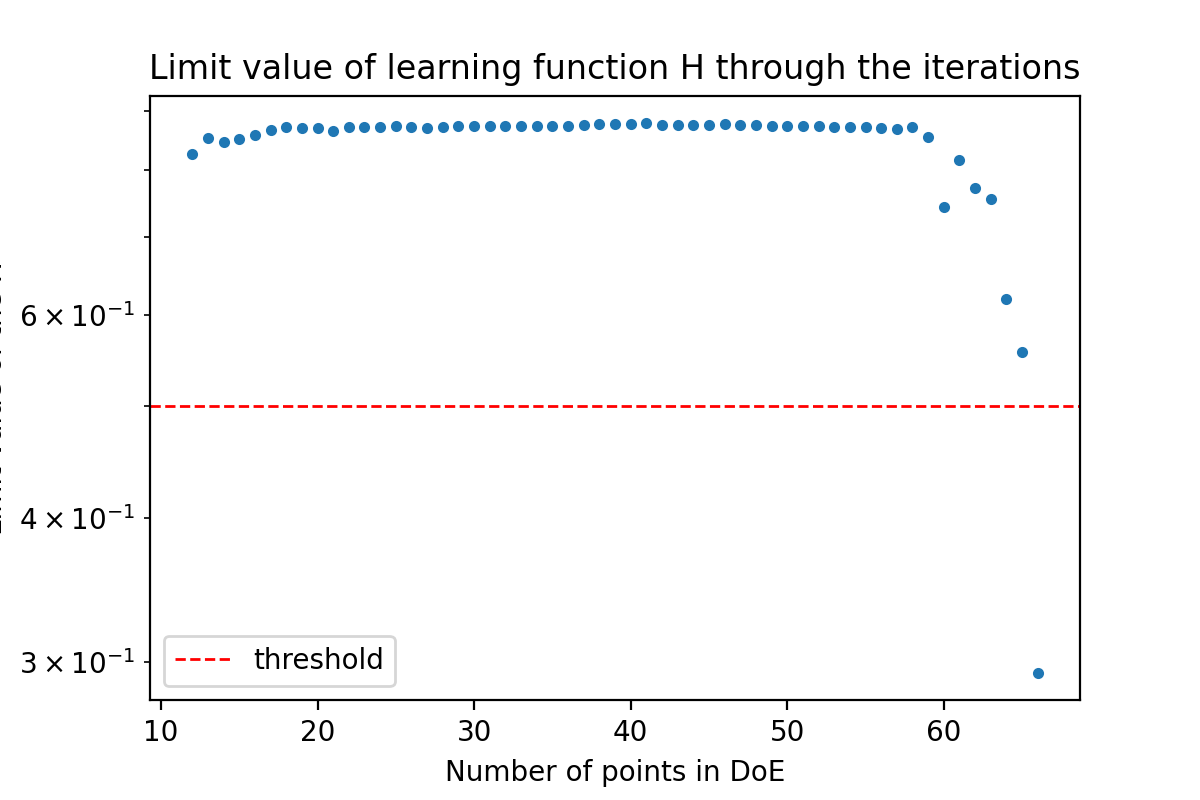
\includegraphics[width=\linewidth]{ex_3_H_lim_values.png}
      \end{subfigure}%
      \caption{Results of example 3}
      \label{fig:ex3_results}
\end{figure*}
\chapter{Conclusion}
The AK-MCS algorithm proved to have several advantages, being a substantial
improvement of the basic MCS method. It retains the advantages of the latter,
improving its main disadvantage which is having to call the expensive performance
function so many times. \\

The choice of one learning function over another should be influenced by the
nature and form of the problem. Although they are all based on the same parameters,
the manner in which they determine the evolution of the prediction process varies
by giving greater importance to different aspects of the design space and the performance
function. Likewise, the choice of thresholds for the stopping conditions is of great importance,
as they represent the usual trade-off between cost and benefit. It could be seen that in
the worked examples, the suggested threshold of the learning function H was too high,
yet for some particular problems it was low enough. \\

Given the simplicity of the nature of the method, its potential for improvement
is very high. In principle, the formulation of new learning functions is a
boundless task. Moreover, different ways of approaching the problem following the
same principles have been studied. For example, in \citep{Peijuan2017} geometrical considerations
are presented that allow to improve the efficiency of the method, although limiting
its applicability. In \citep{Balesdent2013} work is done on a variant of the crude MCS. And as well
as these, there are many modifications that are pending to be studied, and even
proposed, that could further improve the qualities of the method.
\backmatter

%----------------------------------------------------------------------------------------
%	BIBLIOGRAPHY
%----------------------------------------------------------------------------------------

\bibliography{bibliography} % Use the bibliography.bib file for the bibliography
\bibliographystyle{plainnat} % Use the plainnat style of referencing

%----------------------------------------------------------------------------------------

\printindex % Print the index at the very end of the document

\end{document}